%% This is file `elsarticle-template-1-num.tex',
%%
%% Copyright 2009 Elsevier Ltd
%%
%% This file is part of the 'Elsarticle Bundle'.
%% ---------------------------------------------
%%
%% It may be distributed under the conditions of the LaTeX Project Public
%% License, either version 1.2 of this license or (at your option) any
%% later version.  The latest version of this license is in
%%    http://www.latex-project.org/lppl.txt
%% and version 1.2 or later is part of all distributions of LaTeX
%% version 1999/12/01 or later.
%%
%% Template article for Elsevier's document class `elsarticle'
%% with numbered style bibliographic references
%%
%% $Id: elsarticle-template-1-num.tex 149 2009-10-08 05:01:15Z rishi $
%% $URL: http://lenova.river-valley.com/svn/elsbst/trunk/elsarticle-template-1-num.tex $
%%
\documentclass[preprint,12pt]{elsarticle}

%% Use the option review to obtain double line spacing
%% \documentclass[preprint,review,12pt]{elsarticle}

%% Use the options 1p,twocolumn; 3p; 3p,twocolumn; 5p; or 5p,twocolumn
%% for a journal layout:
%% \documentclass[final,1p,times]{elsarticle}
%% \documentclass[final,1p,times,twocolumn]{elsarticle}
%% \documentclass[final,3p,times]{elsarticle}
%% \documentclass[final,3p,times,twocolumn]{elsarticle}
%% \documentclass[final,5p,times]{elsarticle}
%% \documentclass[final,5p,times,twocolumn]{elsarticle}

%% The graphicx package provides the includegraphics command.
\usepackage{graphicx}
%% The amssymb package provides various useful mathematical symbols
\usepackage{amssymb}
\usepackage{amsmath}
%% The amsthm package provides extended theorem environments
%% \usepackage{amsthm}

%% The lineno packages adds line numbers. Start line numbering with
%% \begin{linenumbers}, end it with \end{linenumbers}. Or switch it on
%% for the whole article with \linenumbers after \end{frontmatter}.
\usepackage{lineno}

%% The makecell package adds flexibility to put line breaks in a
%% Table
\usepackage{makecell}
\usepackage{multirow}

%% Outlining package. To be removed when the outline is filled in
\usepackage{outlines}
%% natbib.sty is loaded by default. However, natbib options can be
%% provided with \biboptions{...} command. Following options are
%% valid:

%%   round  -  round parentheses are used (default)
%%   square -  square brackets are used   [option]
%%   curly  -  curly braces are used      {option}
%%   angle  -  angle brackets are used    <option>
%%   semicolon  -  multiple citations separated by semi-colon
%%   colon  - same as semicolon, an earlier confusion
%%   comma  -  separated by comma
%%   numbers-  selects numerical citations
%%   super  -  numerical citations as superscripts
%%   sort   -  sorts multiple citations according to order in ref. list
%%   sort&compress   -  like sort, but also compresses numerical citations
%%   compress - compresses without sorting
%%
%% \biboptions{comma,round}

% \biboptions{}

\journal{Applied Physics Laboratory Digest}

\begin{document}

\begin{frontmatter}

%% Title, authors and addresses

\title{Application of the Hybrid Resilience Framework to a Fleet of
  Aircraft with Emphasis on an Intertemporal Substitutability
  Algorithm with Stakeholder-Defined Values}

%% use the tnoteref command within \title for footnotes;
%% use the tnotetext command for the associated footnote;
%% use the fnref command within \author or \address for footnotes;
%% use the fntext command for the associated footnote;
%% use the corref command within \author for corresponding author footnotes;
%% use the cortext command for the associated footnote;
%% use the ead command for the email address,
%% and the form \ead[url] for the home page:
%%
%% \title{Title\tnoteref{label1}}
%% \tnotetext[label1]{}
%% \author{Name\corref{cor1}\fnref{label2}}
%% \ead{email address}
%% \ead[url]{home page}
%% \fntext[label2]{}
%% \cortext[cor1]{}
%% \address{Address\fnref{label3}}
%% \fntext[label3]{}


%% use optional labels to link authors explicitly to addresses:
%% \author[label1,label2]{<author name>}
%% \address[label1]{<address>}
%% \address[label2]{<address>}

\author{Roy Emanuel II\corref{cor1}}

\address{Maryland, United States}

\begin{abstract}
%% Text of abstract

\end{abstract}
Long-term high capital systems have multiple stakeholders with
misaligned preferences. This study continues development of a hybrid
resilience framework with the intent to allow stakeholders to better
identify their tradespace as compared to normal metrics or where no
current metrics exist. The paper develops a case study of a fleet of
training aircraft with two key stakeholders. Squadron commanders and
program managers. Each stakeholder has its own preference profile
including time horizon, endogenous preference, and intertemporal
substitutability. 

\begin{keyword}
Resilience \sep Simulation \sep Preferences \sep Endogenous Preference
\sep Intertemporal substitution \sep Time horizon
%% keywords here, in the form: keyword \sep keyword

%% MSC codes here, in the form: \MSC code \sep code
%% or \MSC[2008] code \sep code (2000 is the default)

\end{keyword}

\end{frontmatter}

%%
%% Start line numbering here if you want
%%
\linenumbers

%% main text
\section{Motivation}
\label{S:1}

\subsection{Department of Defense Sustainability Problems}

The Department of Defense (DoD) in the United States manages an
incredible number of complicated systems that must operate in austere
and unforgiving environments while being sustained for long periods of
time. Replacement systems are expected to be more capable than
predecessors and often to last longer as well. The difficulties
surrounding DoD acquisition often lead to delays in 
the introduction of the systems. Examples of delayed acquisitions
include the F-35 Joint Strike Fighter
\cite{Werner2018}, the Zumwalt class of destroyers \cite{Katz2018},
the KC-46 tanker aircraft \cite{Mehta2016}, and U.S. Army command and
control systems \cite{Edwards2017}.

Aging systems must operate past
their planned lifetimes to compensate for these delays. This life extension has
reliability, safety, and operational implications. One method to deal
with the problems of aging systems is a System Life Extension
Program (SLEP). A SLEP extends the lifetime and often adds capability
to an aging system. Many government systems are undergoing SLEP including the Army
Tactical Missile System \cite{DOTE2017,zacks2015}, weather radars
\cite{ROC2018}, ships 
\cite{eckstein2018,NAVSEA2018}, and aircraft
\cite{Lockheed2017,Garbarino2018,Tirpak2015,jennings2018}

The U.S. Government recognizes resilience as a key aspect of assuring
mission success.  The DoD
defines mission assurance as ``\ldots a process to 
protect or ensure the continued function and resilience of
capabilities and assets by refining, integrating and synchronizing all
aspects of the DoD \ldots'' \cite{DepartmentofDefense2016a} The
current U.S. National Security  
Strategy prioritizes increased government resilience functions
\cite{Trump2017}. The National Security Strategy builds upon
earlier Presidential Policy Directives defining the future posture of
critical infrastructure systems. \citep{PPD8,PPD21}. 

This study applied a hybrid resilience framework
\cite{Ayyub2014,Ayyub2015,Emanuel2017,Emanuel2018} in the context of
a fictional DoD flight training system. This study developed a
discrete event simulation for the flight operations of a squadron of
aircraft; defined the critical functional outputs of the simulation
in the context of two stakeholders' preferences; and defined
stakeholder preference profiles informed by the key functional outputs
of the system and threats to mission assurance. Stakeholder
preferences profiles include
time horizon, endogenous preference, and intertemporal
substitutability.

The discrete nature of the simulation required
modification of the analytic resilience model used in previous work
\cite{Ayyub2014,Ayyub2015,Emanuel2017,Emanuel2018}.  
Resilience modeling is a tool that can be brought to bear when making 
critical decisions regarding acquisition and lifetime extension of
critical DoD systems. Part of the
hybrid resilience framework is quantification of 
the intertemporal substitutability of system functional output for a
stakeholder. Previous studies  assume a
constant value for intertemporal substitutability
\cite{Emanuel2017,Emanuel2018}. The study  expand the options for
modeling stakeholder intertemporal substitutability. The study
demonstrates the impact of changes to a stakeholder's preference model
to the resilience of the system. 

%% \subsection{Study Content}
%% This paper demonstrates a hybrid resilience framework intended to produce a
%% resilience value for a given course of action in the context of a
%% given stakeholders preferences.

Section~\ref{s:HRF} describes the
resilience framework and the family of models that are linked
together to produce a resilience value for a functional output -
stakeholder preference profile combination. Section~\ref{s:CaseStudy}
describes the system of interest, simulation independent variables, the parameters of
interest in the system, courses of action, and stakeholder preference
profiles. Section~\ref{s:Results} contains the results of the 
simulation and the resilience analytical model. Section~\ref{s:Disc}
provides context for the results and lays out several options for
future work including the system model, stakeholder
models, and incorporation of a benefit-cost framework. 


%% \section{Literature Review}
%% \subsection{SLEP Research}

%% Levin, Kroshl, and Brodfuehrer investigated a methodology for
%% antifragile decision-making.

%% NOAA has a SLEP program for its WSR-88D \cite{ROC2018}.
%% \begin{itemize}
%%   \item Use the Acq folder from mendeley to populate the SLEP and IOC
%%     delay considerations
%% \end{itemize}

%% \subsection{Metrics for Assessing Fleet Health}
%% \subsubsection{Availability}
%% Availability is a measure (check that that is the word) for fleet
%% health. Saleh and Maris \cite{Saleh2006} identify the shift from
%% component based analysis of reliability to quantification of
%% system-level attributes such as availability. 
%% \subsection{Resilience}
%% Brief discussion of some of the metrics that exist, and why they are
%% not good for the study?

\section{Hybrid Resilience Framework}
\label{s:HRF}

%% The reader should refer to Emanuel and Ayyub \cite{Emanuel2018}
%% \emph{in press} for a thorough introduction to the hybrid resilience
%% framework. A brief summary with emphasis on expanded points of the
%% framework.

%% \subsection{Resilience}

The Society for Risk Analysis provides a operational definition of
resilience: \cite{SRA2016}: ``Resilience is the ability of a system to
reduce the initial adverse effects (absorptive capability) of a
disruptive event (stress) and the time/speed and costs at which it
is able to return to an appropriate functionality/equilibrium
(adaptive and restorative capability). The disruptive events maybe
shocking or creeping, endogenous or exogenous.'' This statement
describes the epochs of a cycle of operation, disturbance, and
recovery.

%% Figure~\ref{f:perfTraj} depicts these epochs in the context
%% of system output, performance, or figure-of-merit ($\varphi$), of a
%% disturbed system over time. \emph{resistance} (...sustain...basic
%% functionality...) and \emph{recovery} (...restore its basic
%% functionality...) portion of the plot.

Resilience requires a context. Carpenter \emph{et al.}
\cite{Carpenter2001} summarized the context of resilience in
socio-ecological problems with the question ``... resilience of what
to what?''  Studies in engineering proposed adding ``for whom?'' when
discussing engineered systems \cite{Emanuel2017,Emanuel2018}. 
Ayyub \cite{Ayyub2014a} defined the method for measuring
resilience: ``The resilience of a system\'s function can be measured
based on the persistence of a corresponding functional performance
under uncertainty in the face of disturbances.'' One or multiple
stakeholders' preferences provide the context for assessing the value
of the system's functional output. The stakeholder preferences answer
the questions ``How much is enough?'', ``How long must the system
perform?'', and ``What value will today's surplus output have when the
system suffers a disturbance in functional output?''
\cite{Emanuel2017,Emanuel2018} 

%% \subsection{Generalized Hybrid Model}
The resilience framework, based upon the Class III hybrid model
proposed by Shanthikumar and Sargent \cite{Shanthikumar1983},
comprises the system models, a stakeholder preference model, and a resilience
model. Figure~\ref{f:ResilienceFramework} depicts the
relationships. The hybrid model guides
developing the required functional output data, stakeholder
preferences, and the resilience analytical model. The framework connects  the
outputs of the system of interest (\emph{of what?}), the threats to system
performance (\emph{to what?}),
and the desires of different stakeholders (\emph{for whom?}) to produce a resilience
value that can communicate comparative resilience among options for
 stakeholders with conflicting and concordant preferences.

The hybrid resilience framework guides the analyst through the analysis:
\begin{enumerate}
  \item Identify the system of interest
  \item Identify system representation, for example:
    \begin{itemize}
    \item System in its operating environment
    \item System in a test environment
    \item Surrogate system
    \item System simulation
    \end{itemize}
  \item Collect functional output data, such as:
    \begin{itemize}
    \item Direct measurement from operating system
    \item Direct measurement from test system
    \item Outputs from system simulation
    \end{itemize}
  \item Define stakeholder preference profiles:
    \begin{itemize}
    \item Time horizon
    \item Endogenous preference
    \item Intertemporal substitutability
    \end{itemize}
  \item Produce resilience measurements
\end{enumerate}


\begin{figure}[h]
  \centering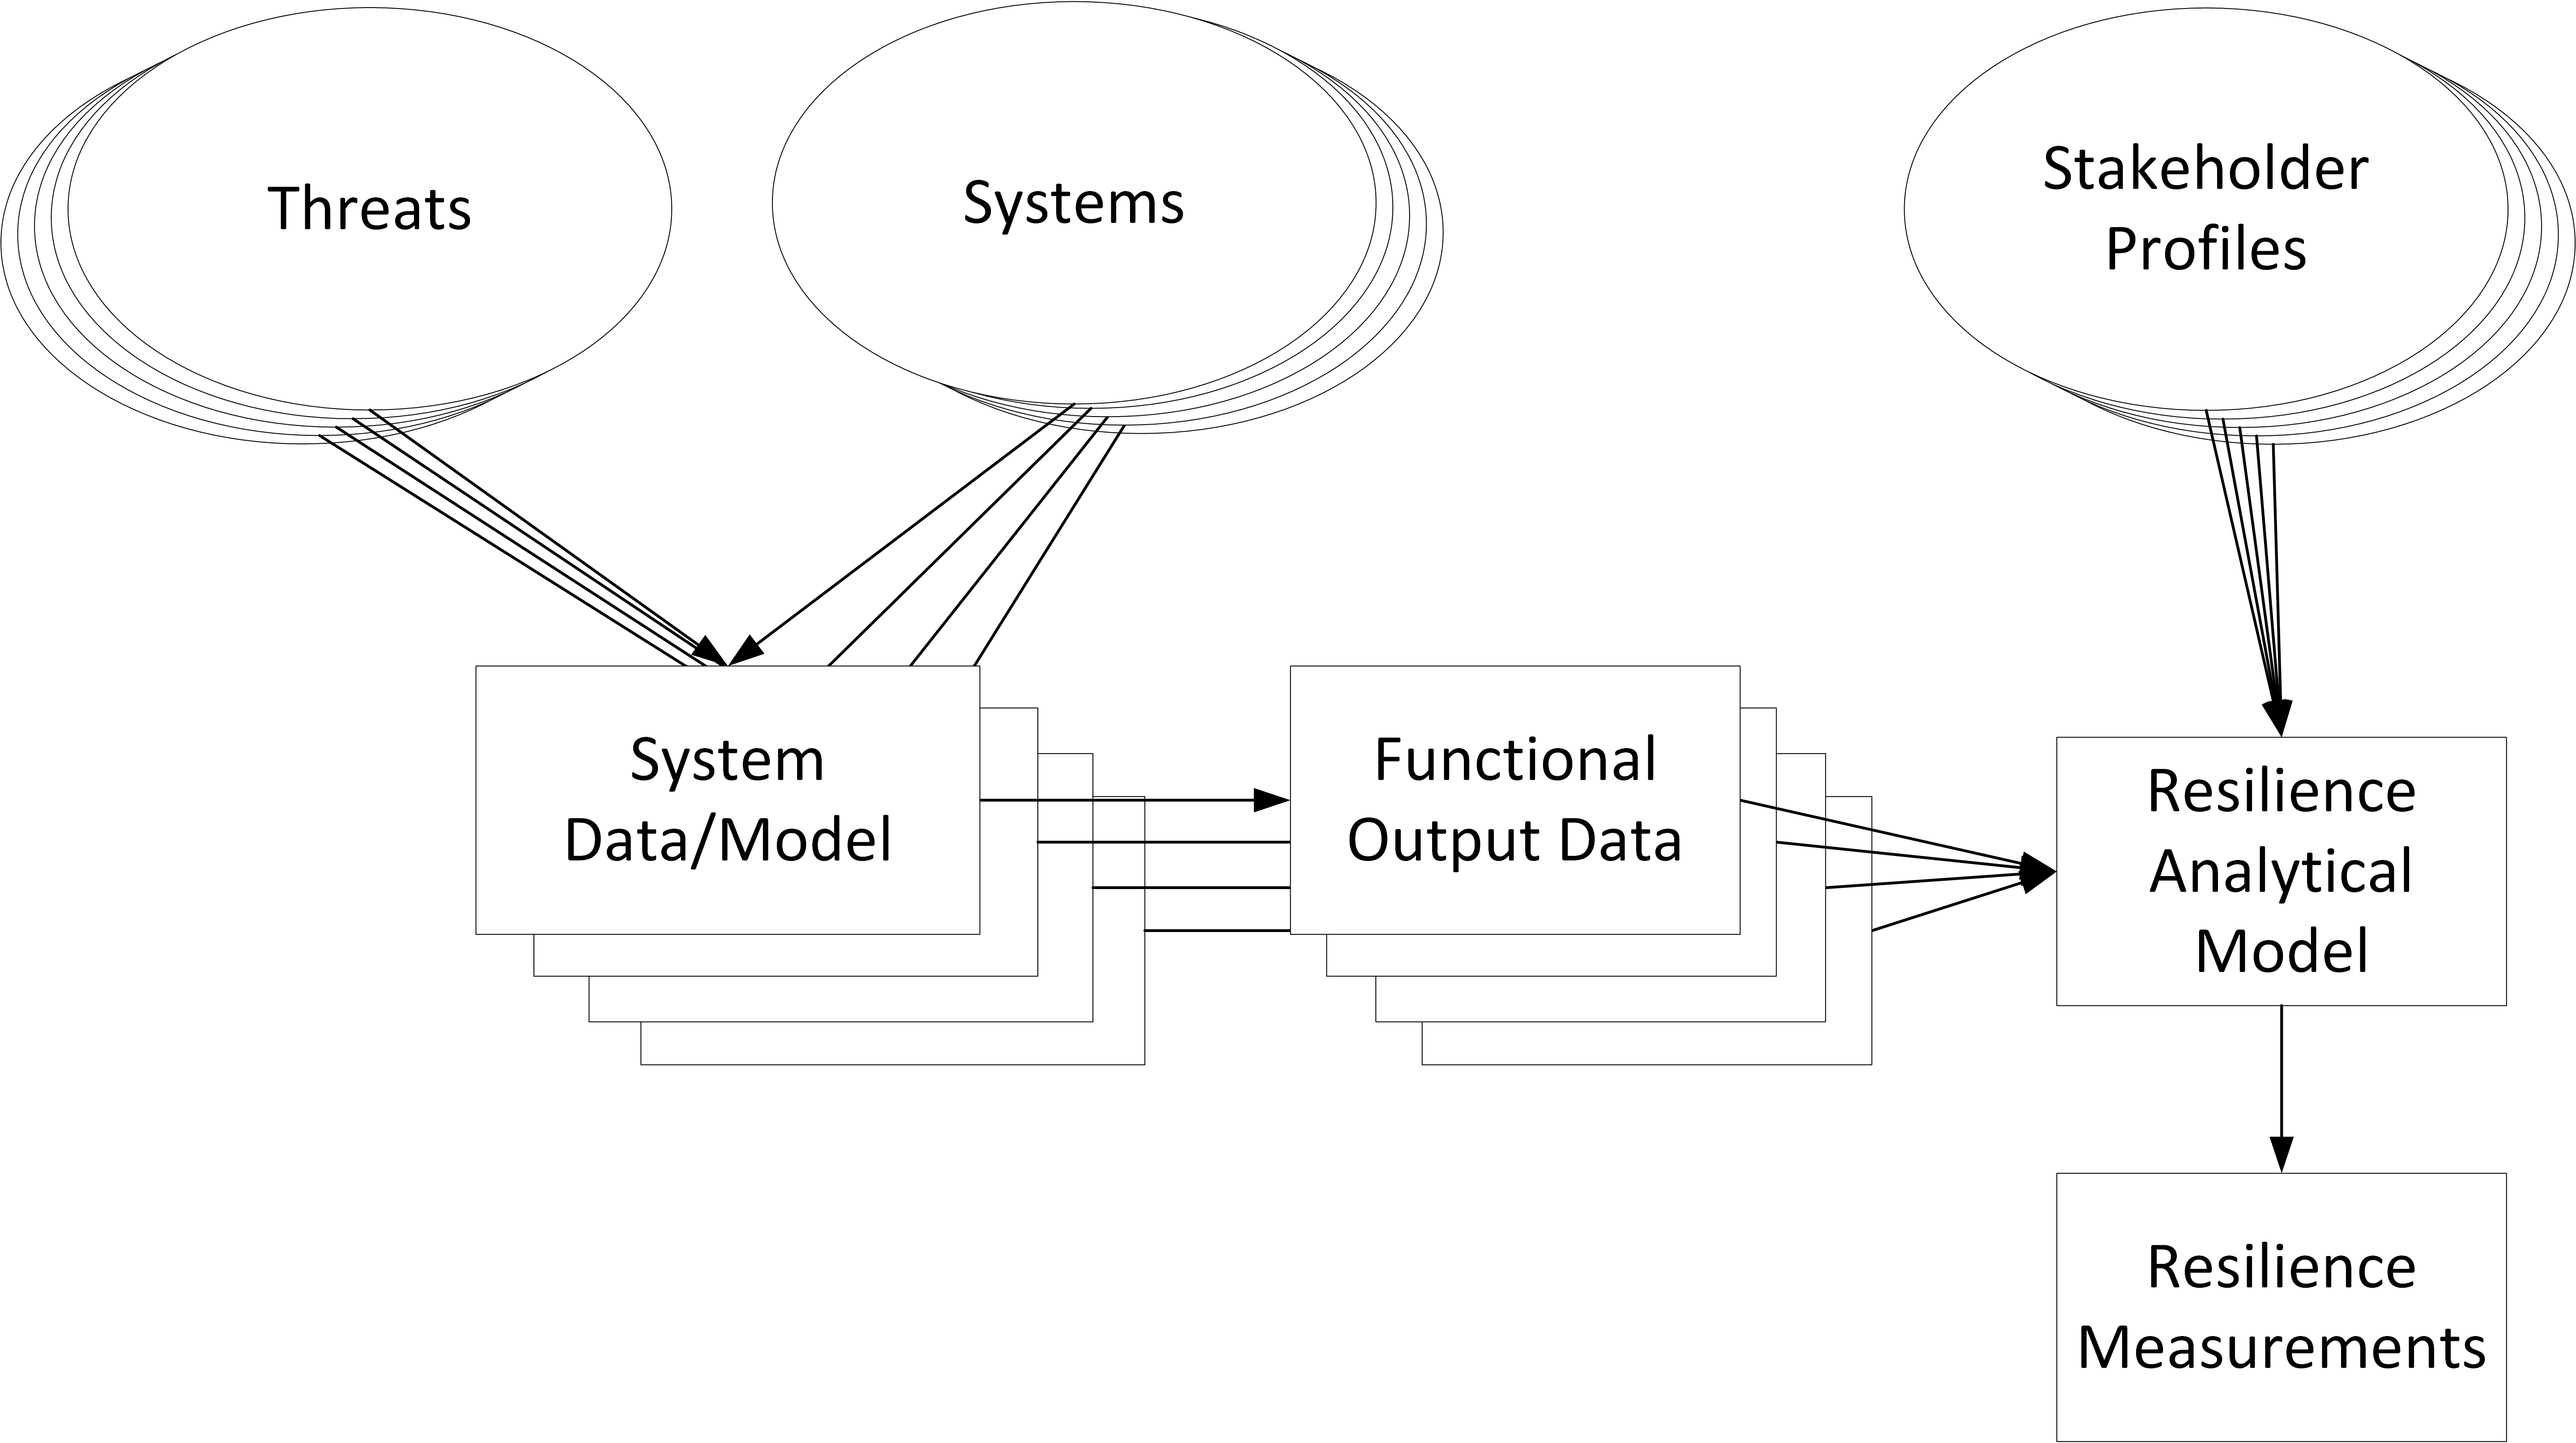
\includegraphics[width=\textwidth]{ClassIII.png}
  \caption{Resilience Framework Relationships Among Models}
  \label{f:ResilienceFramework}
\end{figure}

\subsection{System Identification and Functional Output Measurement}
The analyst first identifies the system(s) of interest and the
functional output(s). This activity sets the scope of the
study which drives the physical and functional definition of the
system(s) of interest. Stakeholders have requirements for output from the
system of interest. Selecting the system and functional models should
always be performed in this context. The analyst defines the external
layers interfacing with the system of interest. The external layers
provide context for the normal operating environment of the system and
disturbance type, frequency, and magnitude to the system \cite{APL2015}.

The functional outputs of the system of interest provide the
measures for the resilience analytic model \cite{Ayyub2014}. The
symbol $\varphi$ represents functional performance. The functional
performance is a key input for the resilience analytical model.

\subsection{Stakeholder Preference Profiles}
The stakeholder preference profiles provides the context for the
functional output data. A stakeholder must determine the quantity of
output that satisfies stakeholder needs, the overall time period the
system must operate to be useful to the stakeholder, and the ability
to time-shift surplus functional output to periods of shortage.

\subsubsection{Stakeholder Preference Profiles: Endogoneous Preference}

Endogeneous preference, $Q$, is the amount of the functional output
that a stakeholder desires at a given time \cite{Black2013}.  Many
models of resilience assume the stakeholder's endogeneous preference
remains constant over time, is equal to the 100\% 
performance level under operating conditions, and does not change
after a disturbance \cite{Emanuel2017}. The hybrid resilience
framework allows for time and disturbance dependent endogeneous
preferences \cite{Emanuel2018}.

\subsubsection{Stakeholder Preference Profiles: Time Horizon}
Time horizon, $t_h$, is the furthest time in the future that a stakeholder 
has interest in an item or process \cite{Black2013}. The concept has a
significant impact on the results 
of a resilience analysis because time 
horizon changes with a change in stakeholder perspective
\cite{Emanuel2018}. Time horizon may also be uncertain in
some cases. In the environment we are discussing, a key source of
uncertainty is the possibility of a delay in a follow-on capability.

\subsubsection{Stakeholder Preference Profiles: Intertemporal
  Substitutability}

Intertemporal substitutability,$\chi$, is the ``replacement of the consumption
of a good or service at one point in time by consumption at a
different time'' \cite{Black2013}. Intertemporal substitutability takes 
values from zero to one. The value of $\chi$ may be constant for the
entire time horizon, or it may be dependent upon time or events. Two
special values of $\chi$ are the \emph{ephemeral} and \emph{permanent}
cases. The \emph{ephemeral} case ($\chi = 0$) allows no substitution across
time. When the system has a shortage at time $t_j$, surplus from time
$t_i$ has no value. The  \emph{permanent} case ($\chi = 1$) where a
surplus retains its full value or utility throughout the time
horizon. Any surplus at time $t_i$ has full value at time $t_j$.



The \emph{adjacent}
case for intertemporal substitutability ``transfers'' surplus from adjacent
time steps into a time step with a shortfall. The surplus-to-shortfall
``transfers'' surplus some number steps before or after 
the shortfall to compensate for the shortfall. The ``transfer'' level may be moderated by a
coefficient that decreases the value of substitution as $t_n$ moves
further away from the time at shortfall.  Intertemporal
substitutability $\chi$ becomes a scalar two-column matrix of an
arbitrary length (For example see Table~\ref{t:chiVec}). The first
column is an index $j$ defining the amount 
of steps from the shortfall that is transferable. The second column is
the fraction of the surplus that is transferable. For example (Table~\ref{t:chiVec}),
 75\% of surplus occurring one time step after shortfall is available
 to transfer while 100\% of surplus one time step before the shortfall
 is available to transfer.


\begin{table}[h]
  \centering
  \begin{tabular}{c l }
    \hline
    \hline
    \textbf{j} & $\mathbf{\chi_j}$ \\
    \hline
    3 & 0 \\
    2 & 0.25 \\
    1 & 0.75 \\
    -1 & 1 \\
    -2 & 0.5 \\
    -3 & 0.25 \\
    -4 & 0.1 \\
    -5 & 0 \\
    \hline
  \end{tabular}
  \caption{Example of the $\chi$ matrix}
  \label{t:chiVec}
\end{table}

\noindent  The following proposed algorithm applies a
surplus to shortfall substitution for an arbitrary number of steps away from the performance
shortfall. The algorithm assumes the surpluses closest in time to the
shortfalls are first to
transfer. Figures~\ref{f:Chi2-1},~\ref{f:Chi2-2},~\ref{f:Chi2-3},~\ref{f:Chi2-4},~\ref{f:Chi2-5},~\ref{f:Chi2-6}
demonstrate the 
algorithm for surpluses 
occurring before the shortfall. 

\begin{enumerate}
\item Define the indices ($j$) and the fraction of substitutability
  ($\chi_j$) for the intertemporal substitutability matrix.
\item Find a performance shortfall, $\varphi_t < Q_t$. This defines
  the time $t$ of the shortfall 
\item Calculate the transferable surplus from the closest index ($j$) before the
  shortfall, $\psi_{t,j} = \chi_{j}(\varphi_{t-j}-Q_{t-j})$
\item If $\varphi_t + \psi_{t,j} < Q_t$,
  \begin{enumerate}
  \item set $\varphi_t:\varphi_t + \psi_{t,j}$ and
    $\varphi_{t-j}:Q_{t-j}$.
  \item Return to Step 2.
  \end{enumerate}
\item If $\varphi_t + \psi_{t,j} \geq Q_t$,
  \begin{enumerate}
  \item Set $\varphi_t:Q_t$
  \item Remove the transferred surplus from
    $\varphi_{t-1} : Q_t + \frac{\psi_{t,j} - (Q_t -
    \varphi_t)}{\chi_{j}}$.
  \item  Return to Step 3 with $j$ one step further from the current
    replacement step.
  \end{enumerate}
\item If $\varphi_t<q_t$ and no surplus remains, return to Step 3
  and apply surplus occurring after the shortfall.
\item When all \emph{available} surpluses are exhausted, set $\varphi$
  for all remaining surpluses to $Q_t$. This step ensures that
  the resilience analytic model does not incorporate inaccessible surpluses. 
\end{enumerate}
    

 
\begin{figure}[h]
  \centering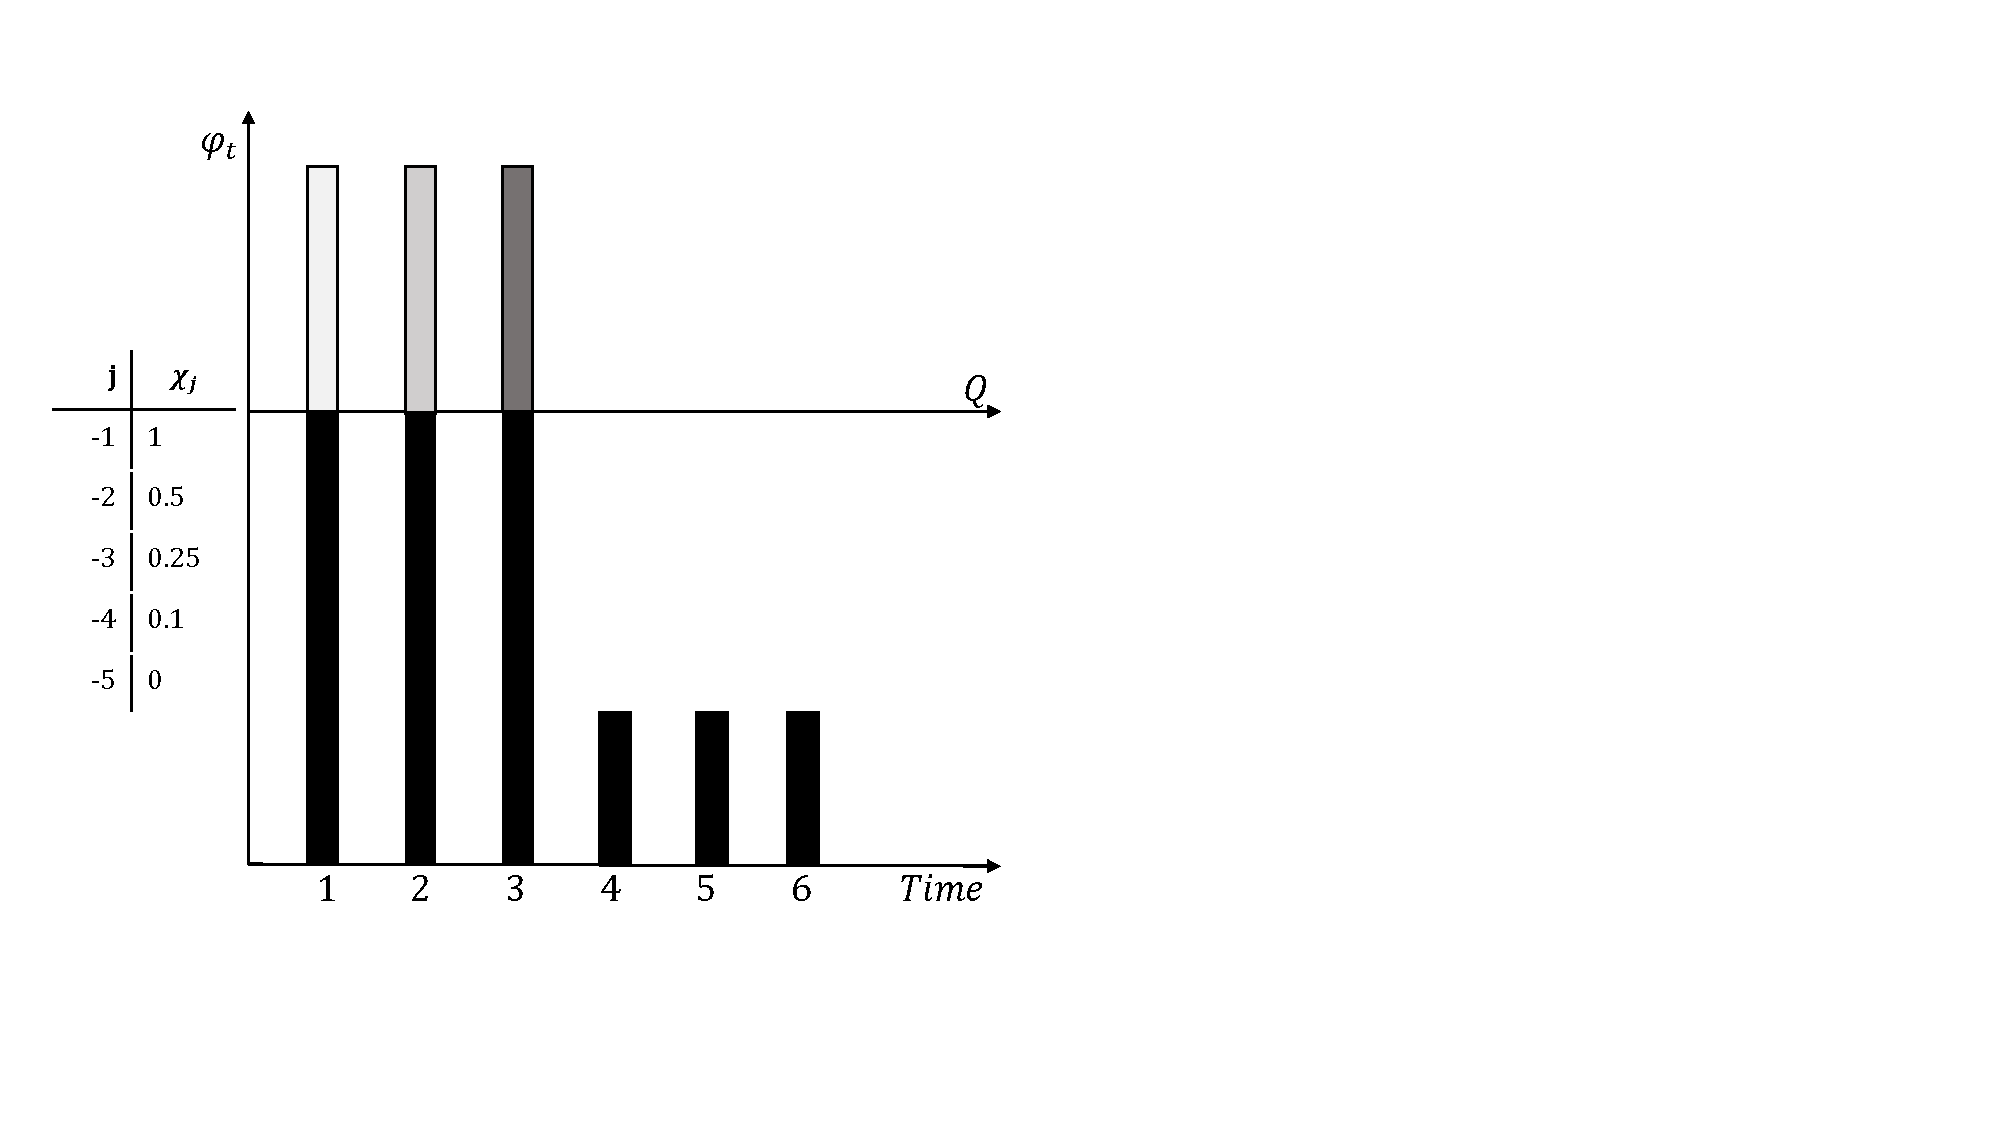
\includegraphics[width=\textwidth]{Chi2-1.pdf}
  \caption{Intertemporal Substitutability Algorithm Example: Define
    the $\chi$ Matrix - The left portion of the figure defines
    the $\chi$ matrix (Step 1). The first shortfall occurs at
    $t=4$ (Step 2)}
  \label{f:Chi2-1}
\end{figure}


\begin{figure}[h]
  \centering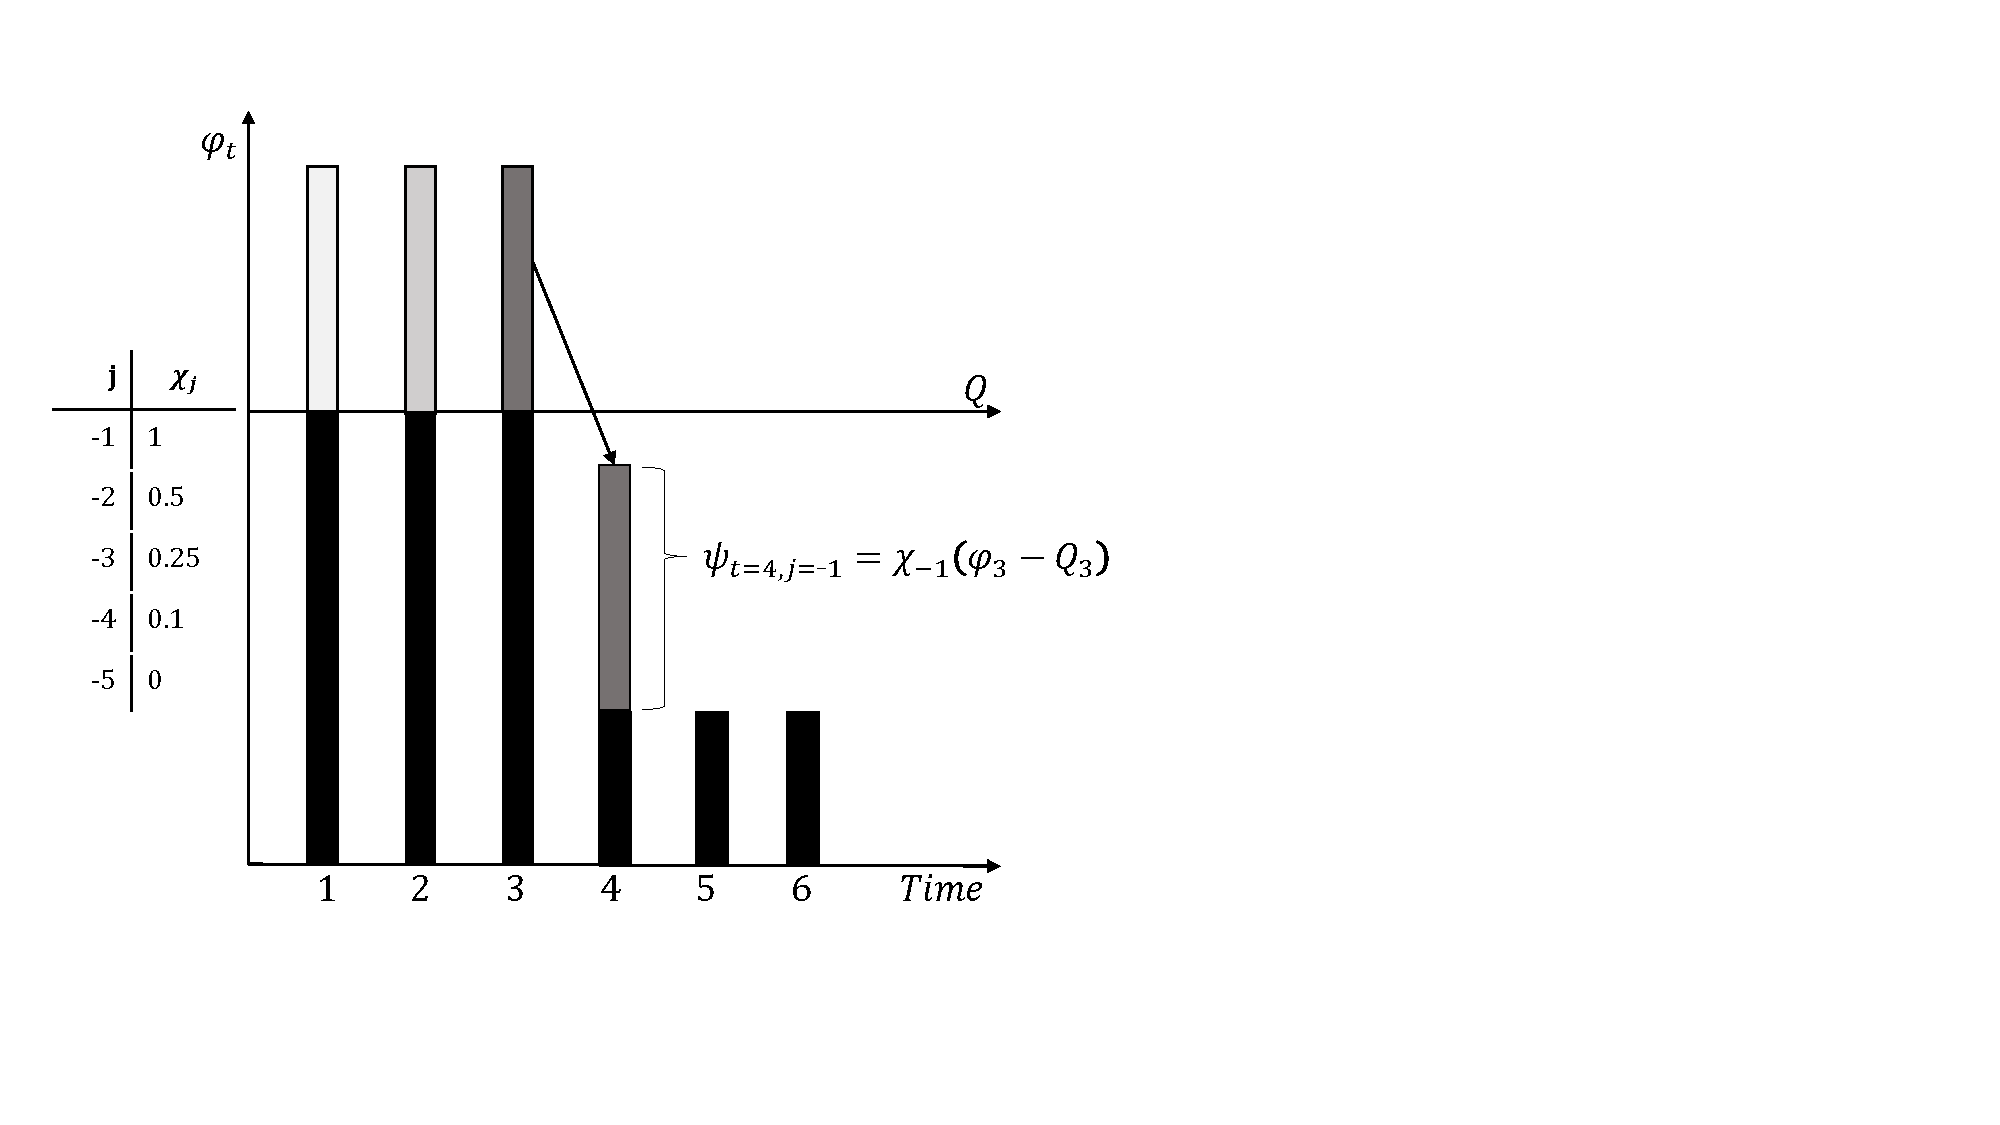
\includegraphics[width=\textwidth]{Chi2-2.pdf}
  \caption{Intertemporal Substitutability Algorithm Example: Transfer
    the Closest Surplus and Assess - The available surplus is $\psi$
    applied to $t=4$ using $j={-1}$ (Step 3)}
  \label{f:Chi2-2}
\end{figure}


\begin{figure}[h]
  \centering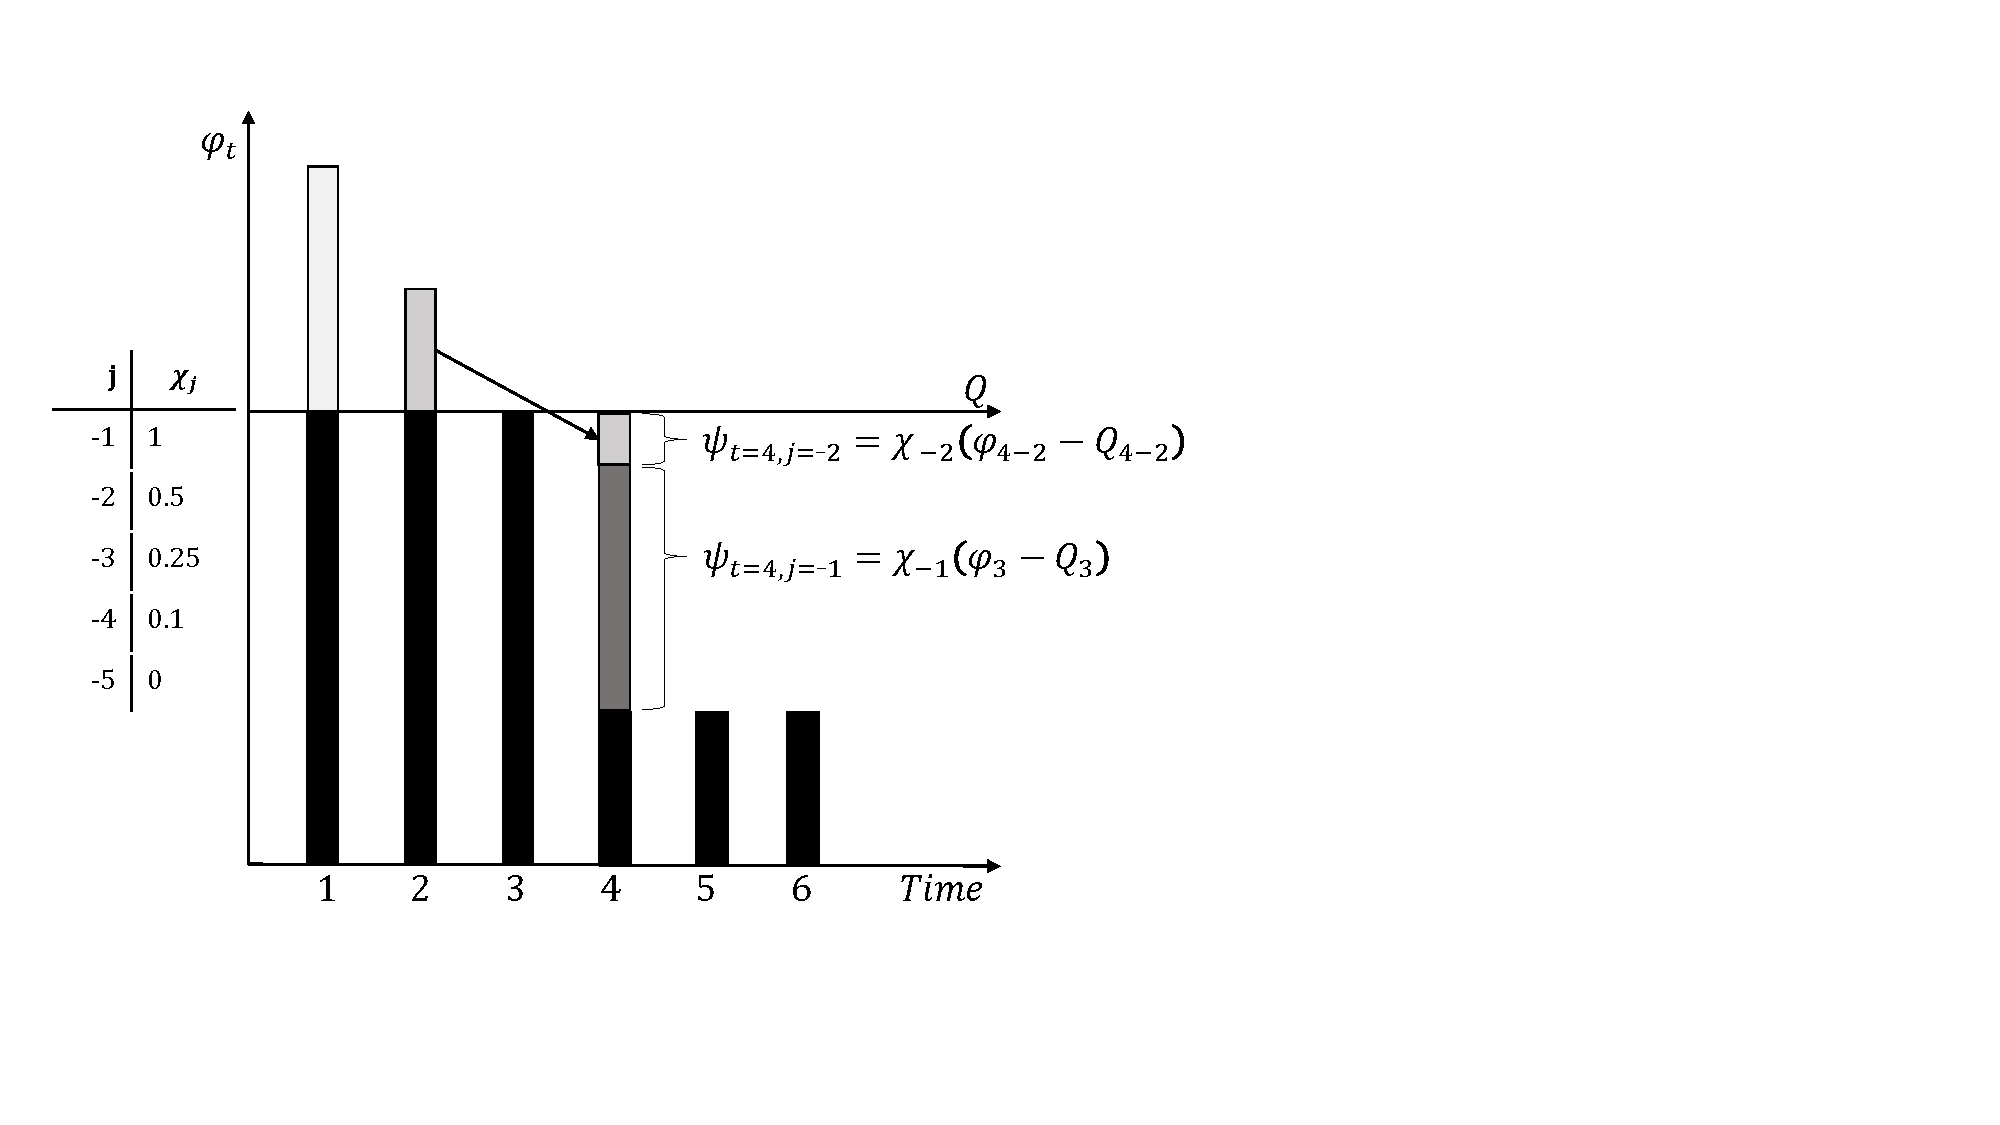
\includegraphics[width=\textwidth]{Chi2-3.pdf}
  \caption{Intertemporal Substitutability Algorithm Example: Transfer
    the Next Closest Surplus and Assess - The surplus from $t=3$ is
    not enough to overcome the shortfall (Step 4), so this transfer
    expends all surplus from $t=3$ (Step 4a), and the algorithm
    transfers surplus one step further from $t=4$ (Step 3)}
  \label{f:Chi2-3}
\end{figure}


(Figure~\ref{f:Chi2-4})
\begin{figure}[h]
  \centering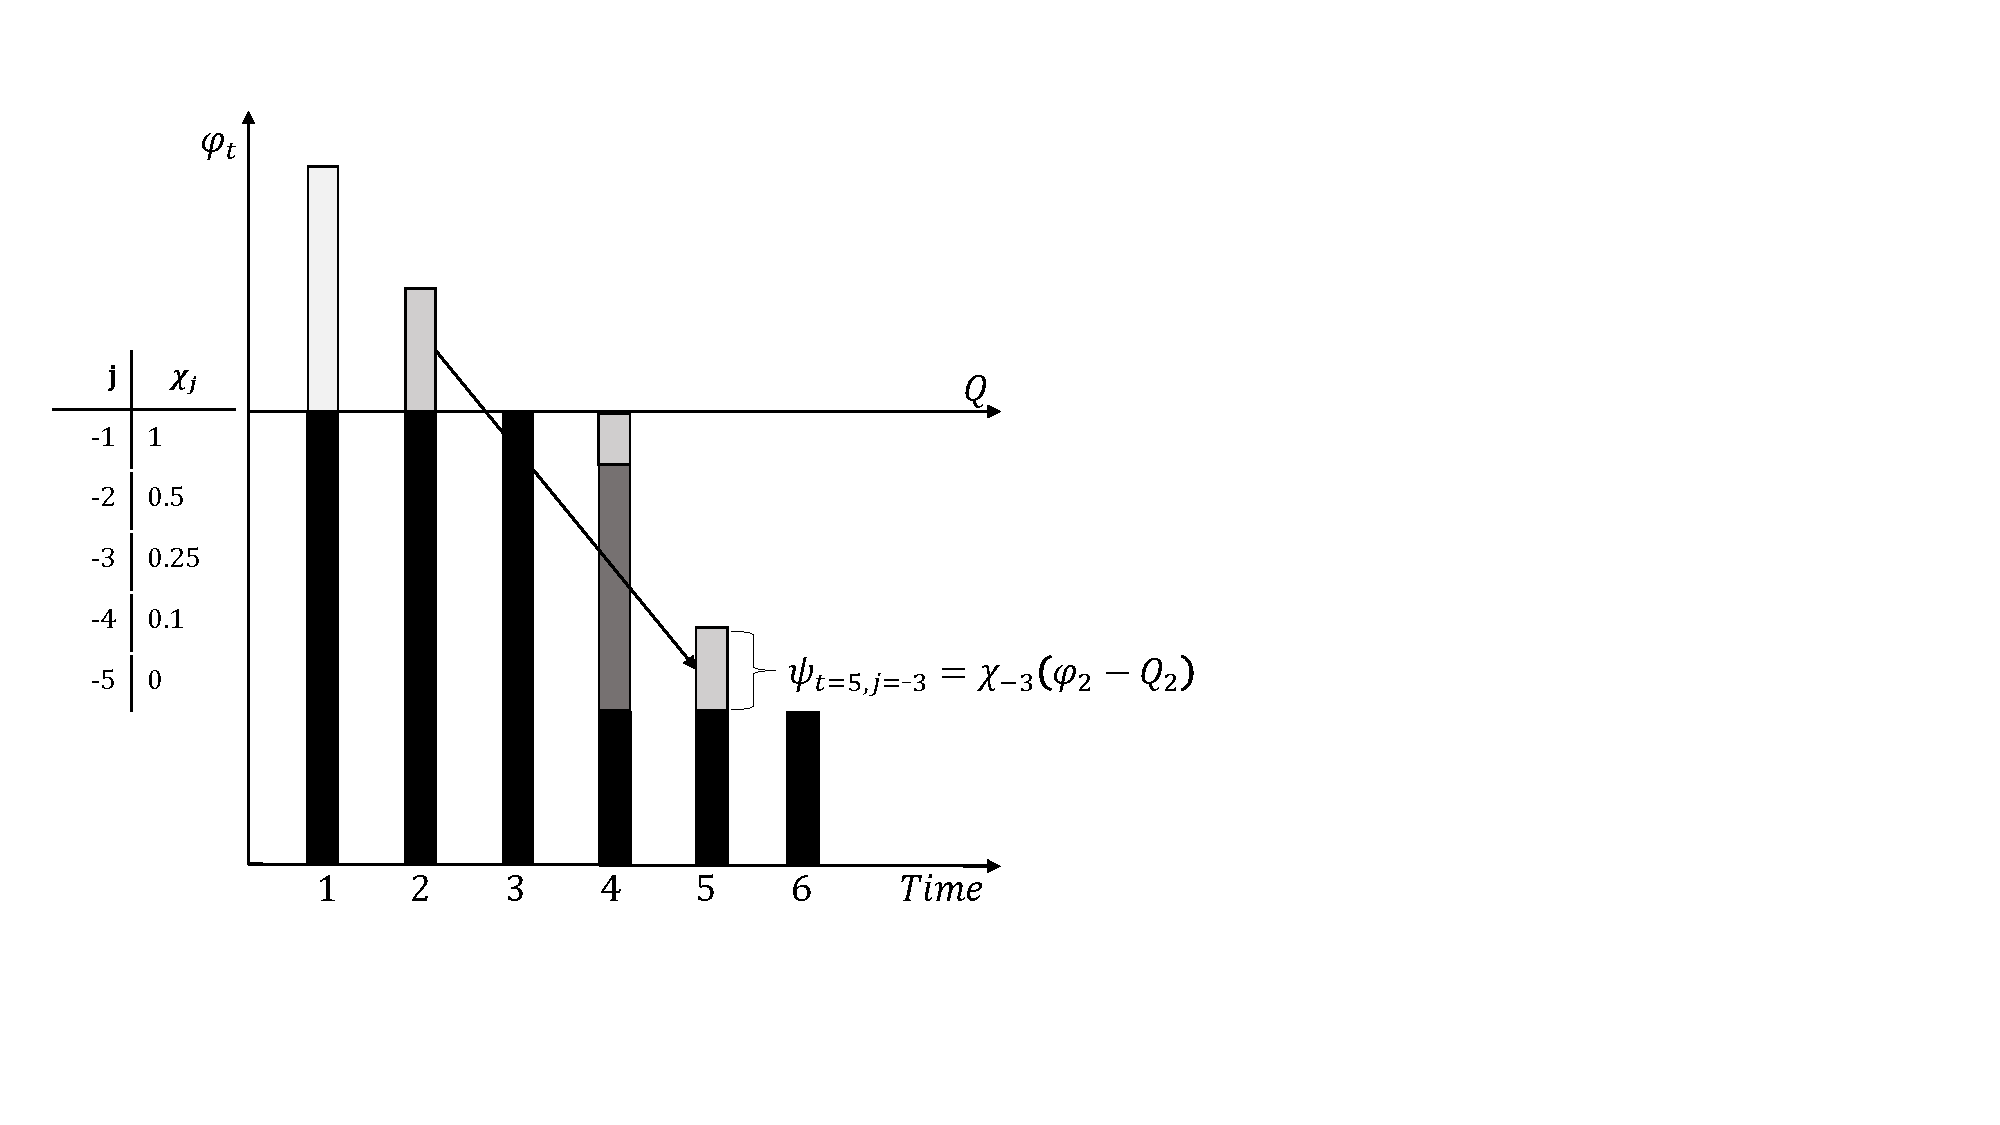
\includegraphics[width=\textwidth]{Chi2-4.pdf}
  \caption{Intertemporal Substitutability Algorithm Example: Find the
    Next Shortfall and Begin Surplus Transfers - This transfer
    satisfies the shortfall and leaves a fraction of the surplus at
    $t=2$ remaining (Step5). With $t=4$ satisfied, the algorithm finds
    the next shortfall at $t=5$. The first two steps have no surplus,
    so the algorithm transfers surplus three steps from $t=5$. This
    exhausts the surplus from $t=2$}
  \label{f:Chi2-4}
\end{figure}
(Figure~\ref{f:Chi2-5}). 
\begin{figure}[h]
  \centering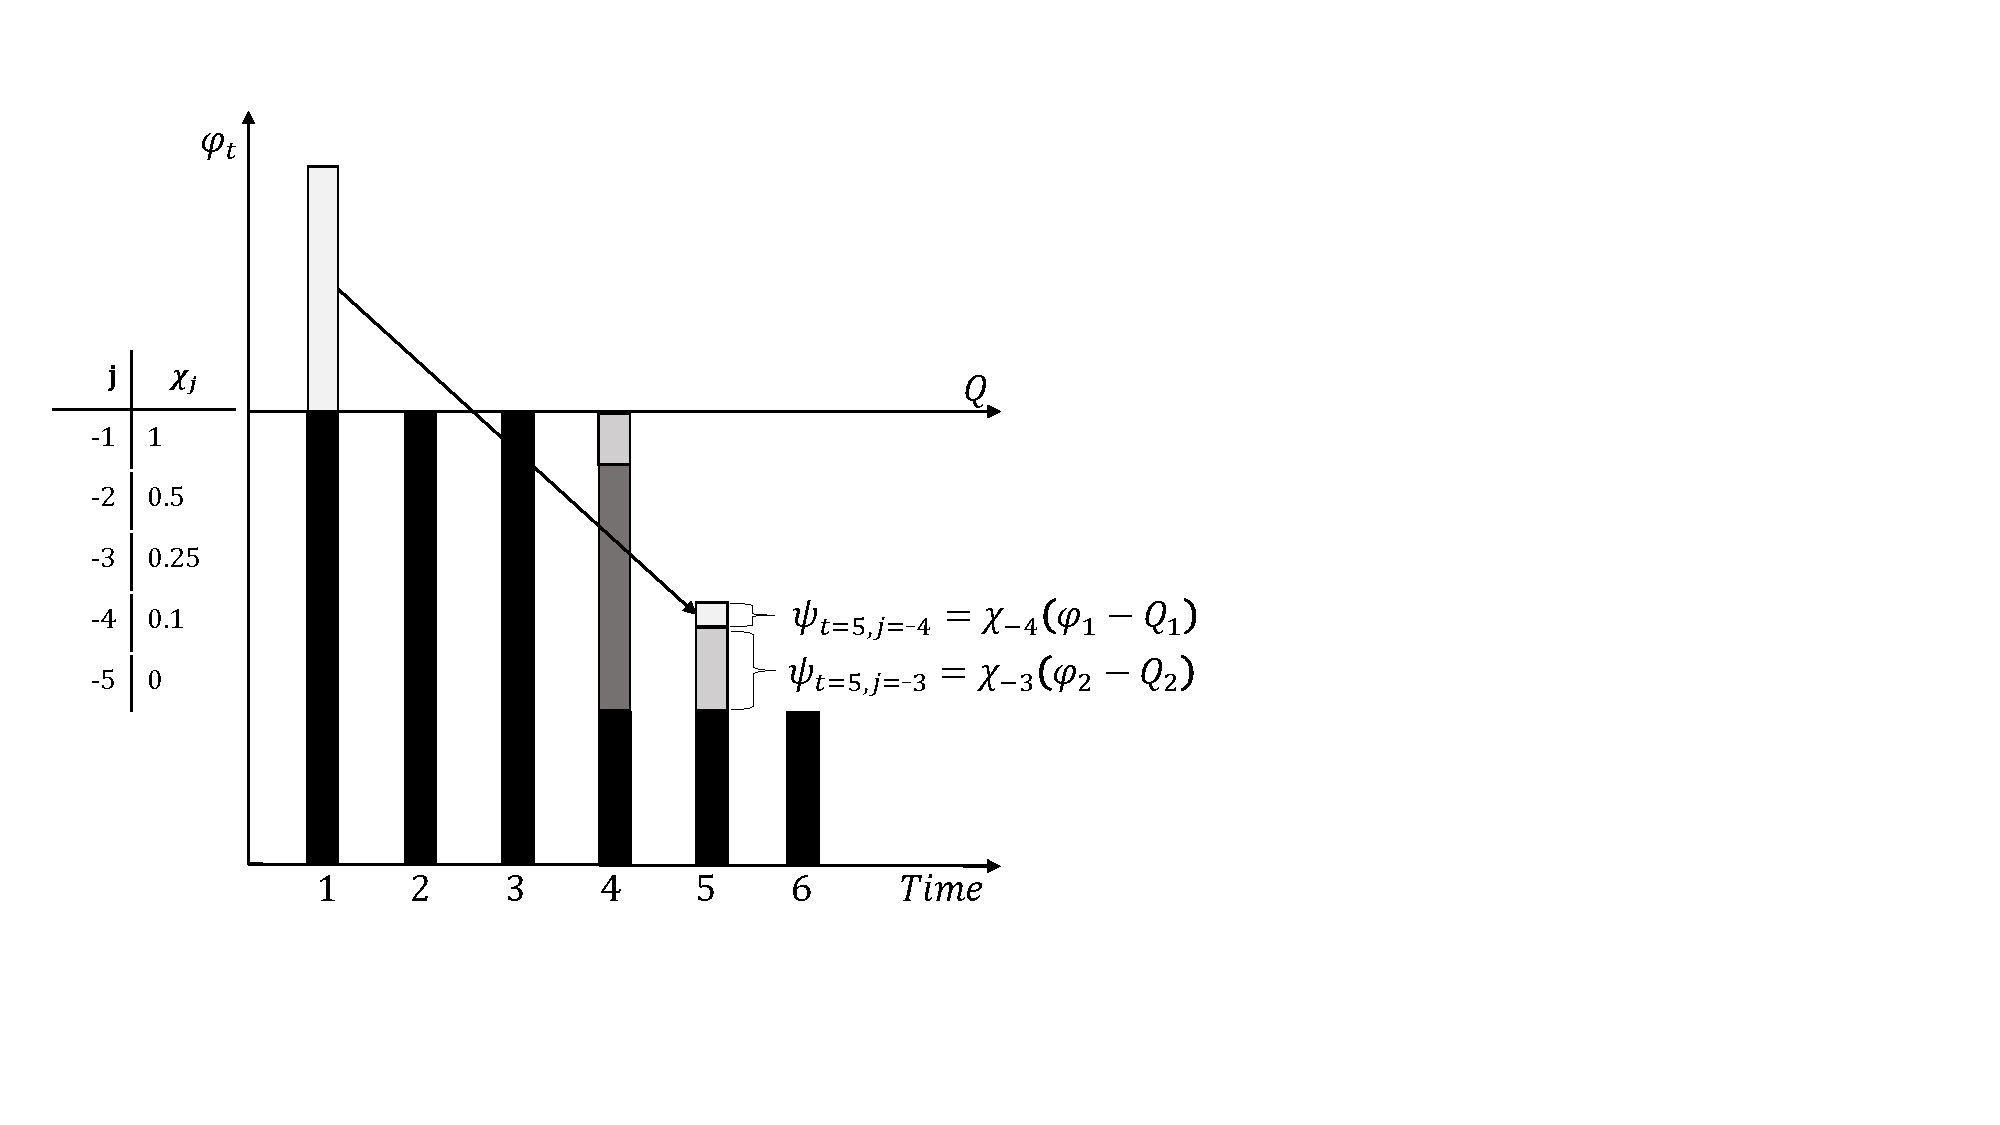
\includegraphics[width=\textwidth]{Chi2-5.pdf}
  \caption{Intertemporal Substitutability Algorithm Example: Execute
    the Final Available Transfer - The surplus from $t=1$ transfers to
    $t=5$}
  \label{f:Chi2-5}
\end{figure}



\begin{figure}[h]
  \centering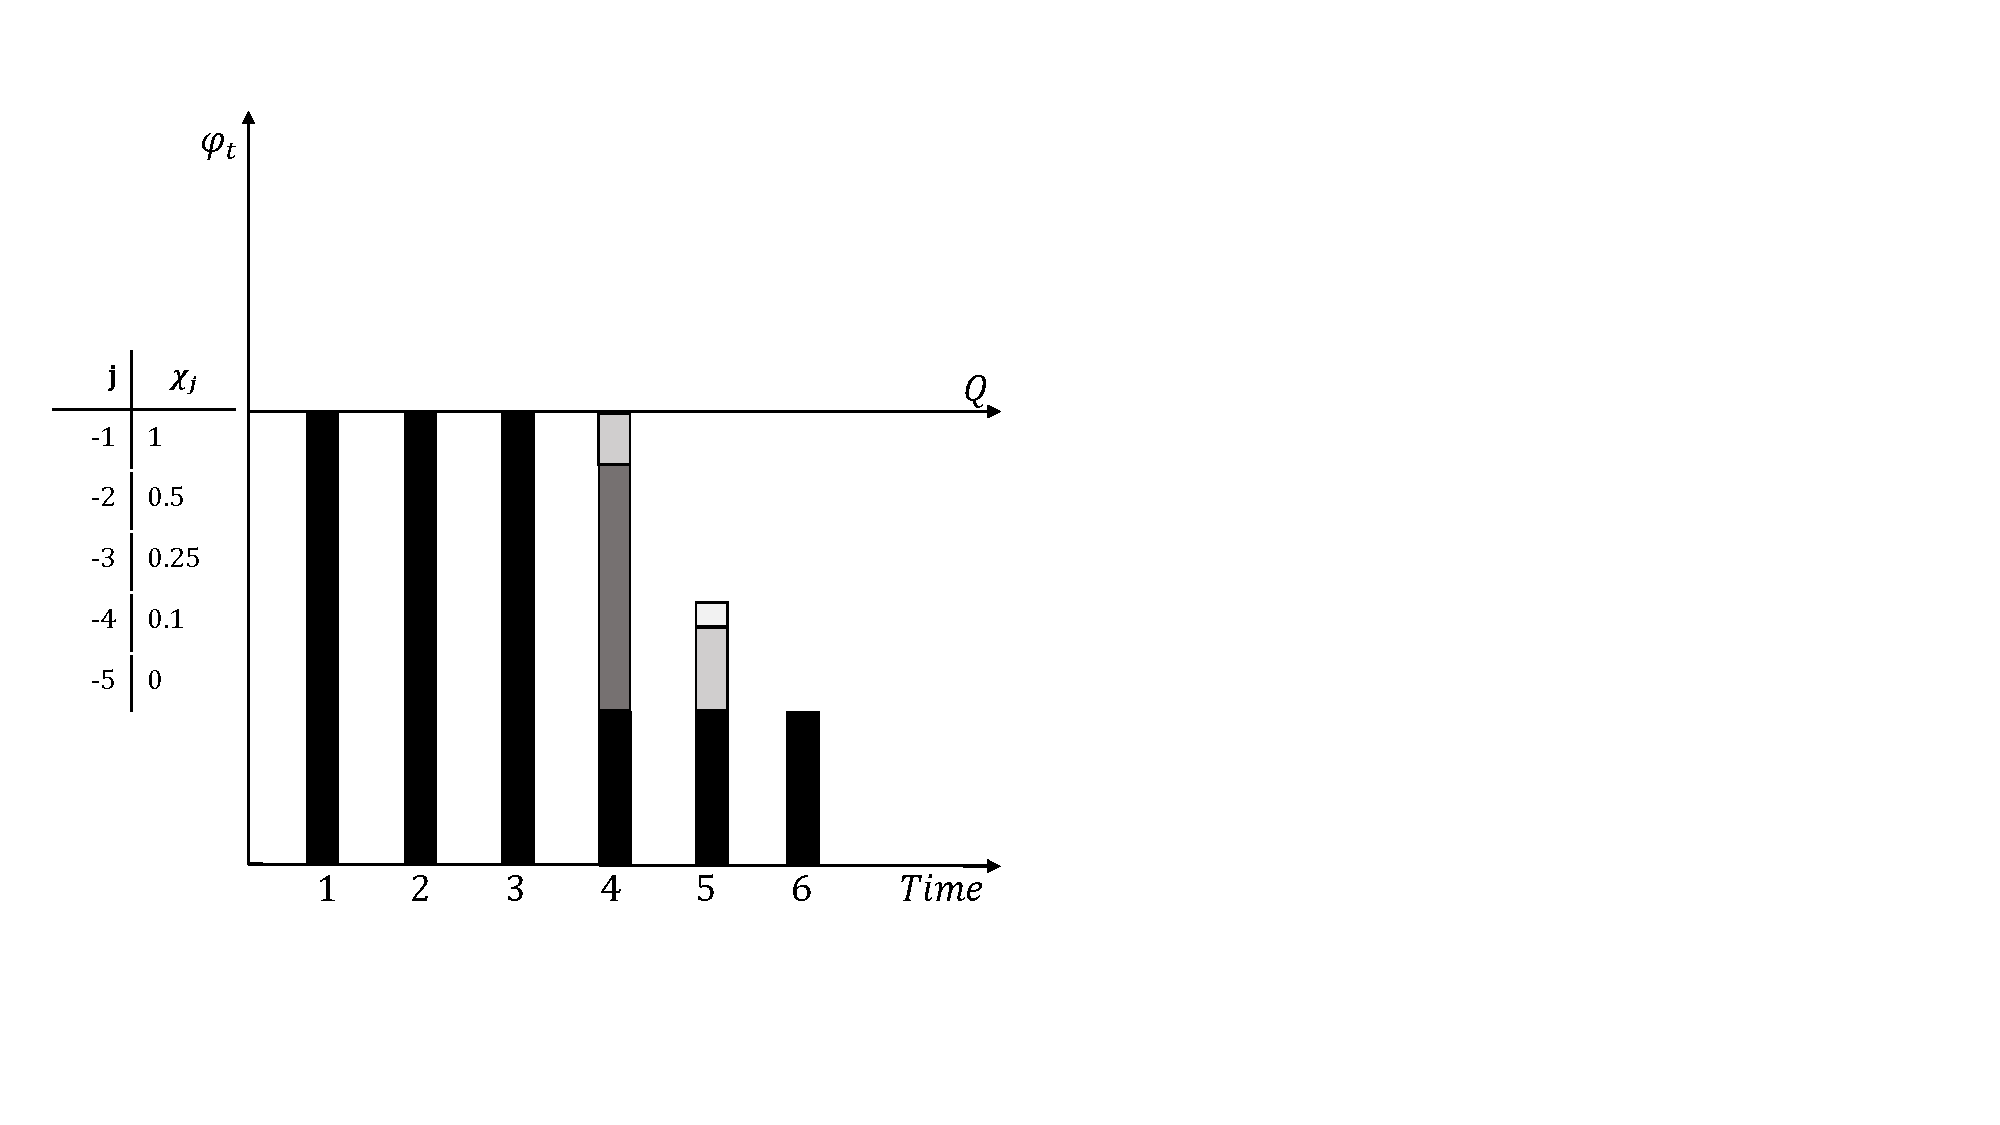
\includegraphics[width=\textwidth]{Chi2-6.pdf}
  \caption{Intertemporal Substitutability Algorithm Example: Modified
    Functional Output with All Surpluses Exhausted - The shortfall at
    $t=5$ cannot be overcome by available surplus, so the algorithm
    ends with the modified functional output shown above.}
  \label{f:Chi2-6}
\end{figure}

This is one example of how the algorithm could
end. This performance is the input for the resilient
analytical model when employing \emph{adjacent} intertemporal
substitutability. 

\subsection{Resilience Analytical Model}


Ayyub \cite{Ayyub2014a} defined the model for resilience used for
this study. Efforts by Emanuel and Ayyub
\cite{Emanuel2017,Emanuel2018} further develop the resilience model
to prepare it to incorporate the outputs of the stakeholder preference
model. The analytical resilience model is:
\begin{equation}
  \label{e:contResilience}
    R = \frac{M_{\chi} \Delta T_i + F_{\chi} \Delta T_f + R_{\chi}
    \Delta T_r + H_{\chi} \Delta T_h}
  {\Delta T_i + \Delta T_f + \Delta T_r + \Delta T_h}
\end{equation}
where the factors $M_{\chi}$, $F_{\chi}$, etc., for continuous system are:
\begin{equation}
  \label{e:RPC}
  F_{\chi}(t) = \left\{\begin{array}{rcl}
      \frac{\displaystyle\int_{t_i}^{t_f}\varphi(t)dt}{\displaystyle\int_{t_i}^{t_f}Q(t)dt}
      & \text{ for } & \varphi(t) \leq Q(t) \\
      1 + \chi(t)
      \frac{\displaystyle\int_{t_i}^{t_f}\varphi(t)-Q(t)dt}{\displaystyle\int_{t_i}^{t_f}Q(t)dt}
      & \text{ for } & \varphi(t) > Q(t)
      \end{array}\right.
\end{equation}

The next task is to develop a discrete representation of the
above. The overal equation for resilience, $R$, remains unchanged, but
the equations for each profile must be modified incorporating
Equation~\ref{e:contResilience}.

\begin{equation}
  \label{e:RPD}
  F_{\chi,t} = \left\{\begin{array}{rcl}
    \frac{\displaystyle\sum_{\tau=t_{i}}^{t_f}\varphi_{\tau}}{\displaystyle\sum_{\tau=t_i}^{t_f}Q_{\tau}}
    & \text{ for } &
    \varphi_{t} \leq Q_t \\
      1 + \chi_t
      \frac{\displaystyle\sum_{\tau = t_i}^{t_f}\varphi_{\tau}-Q_{\tau}}{\displaystyle\sum_{\tau = t_i}^{t_f}Q_{\tau}}
      & \text{ for } &
      \varphi_{t} > Q_{t}
  \end{array}\right.
\end{equation}




Table~\ref{t:StakeParameters} describes the parameters in the
stakeholder performance profile with their respective symbols and
description.

\begin{table}[h]
  \centering
  \begin{tabular}{l c l}
    \hline
    \hline
    \textbf{Name} & \textbf{Symbol} & \textbf{Description} \\
    \hline
    Time horizon &
    $t_h$ &
    \makecell[l]{The latest time that a stakeholder \\
              is interested in system output} \\
    Endogenous preference &
    $q_t$ &
    \makecell[l]{Output desired by stakeholder\\
              at time $t$} \\
    \makecell[l]{Intertemporal\\substitutability} &
    $\chi$ &
    \makecell[l]{the fraction of surplus output \\
              at time $t-t_i$ that is available \\
              to satisfy a shortfall at time $t$}\\
    \hline
  \end{tabular}
  \caption{Components of the Stakeholder Preference Profile}
  \label{t:StakeParameters}
\end{table}

\section{Case Study: Training Squadron of Aircraft}
\label{s:CaseStudy}
The introduction established the current DoD challenges regarding
aging systems and delayed acquisitions\cite{Burgess2015,LaGrone2016,awstf35}. One solution, SLEP of the
aging system, can mitigate a host of problems: 
\begin{itemize}
\item Parts obsolescence \cite{Tomczykowski2001}
\item Part wear-out \cite{jennings2018}
\item Capability improvement \cite{Burgess2015}
\end{itemize}

The decisions for SLEP include systems to modify, amount of life to add, number of
systems to SLEP, and when the SLEP should occur. The impact of the
decisions often occur well beyond the career lifetimes of the people
who make them. Considering the time horizon of the individuals is important.

This case study is based upon current jet trainers (T-45 Goshawk and
T-38 Talon) in the U.S. Navy and U.S. Air Force. These aircraft, along
with instructor pilots, provide training to prepare pilots for flying advanced tactical
aircraft. Trainer aircraft require less maintenance, and less cost
than tactical aircraft. The T-X aircraft is the
oft-delayed replacement for the T-38 \cite{Mehta2013}. No replacement
yet exists for the T-45; The T-45 is undergoing SLEP to increase its operational
lifetime. The T-45 SLEP includes detailed inspections, preventive parts 
replacement, corrosion control, and crack control \cite{jennings2018}.

When possible, the study used unclassified US Navy documents
available via official DoD websites to guide development of the
simulation. In cases where information is missing, the authors made
simulation decisions consistent with personal experience and with the
goal of making the simulation tractable.

Figure~\ref{f:FleetFramework} depicts the hybrid resilience framework
for the training squadron case study. The system of interest is the
training squadron comprising aircrew and aircraft. Threats to the
system are a delay in a replacement aircraft and a surge in graduate
production. The stakeholders share the graduation per quarter and
satisfaction rate functional outputs. Program managers are also
concerned with the daily aircraft availability. The stakeholders have
different preference profiles (time horizon, endogenous preference,
and intertemporal substitutability) for each functional output. The
resilience analytical model calculates resilience of each functional
output-stakeholder preference pairing.

\begin{figure}[h]
  \centering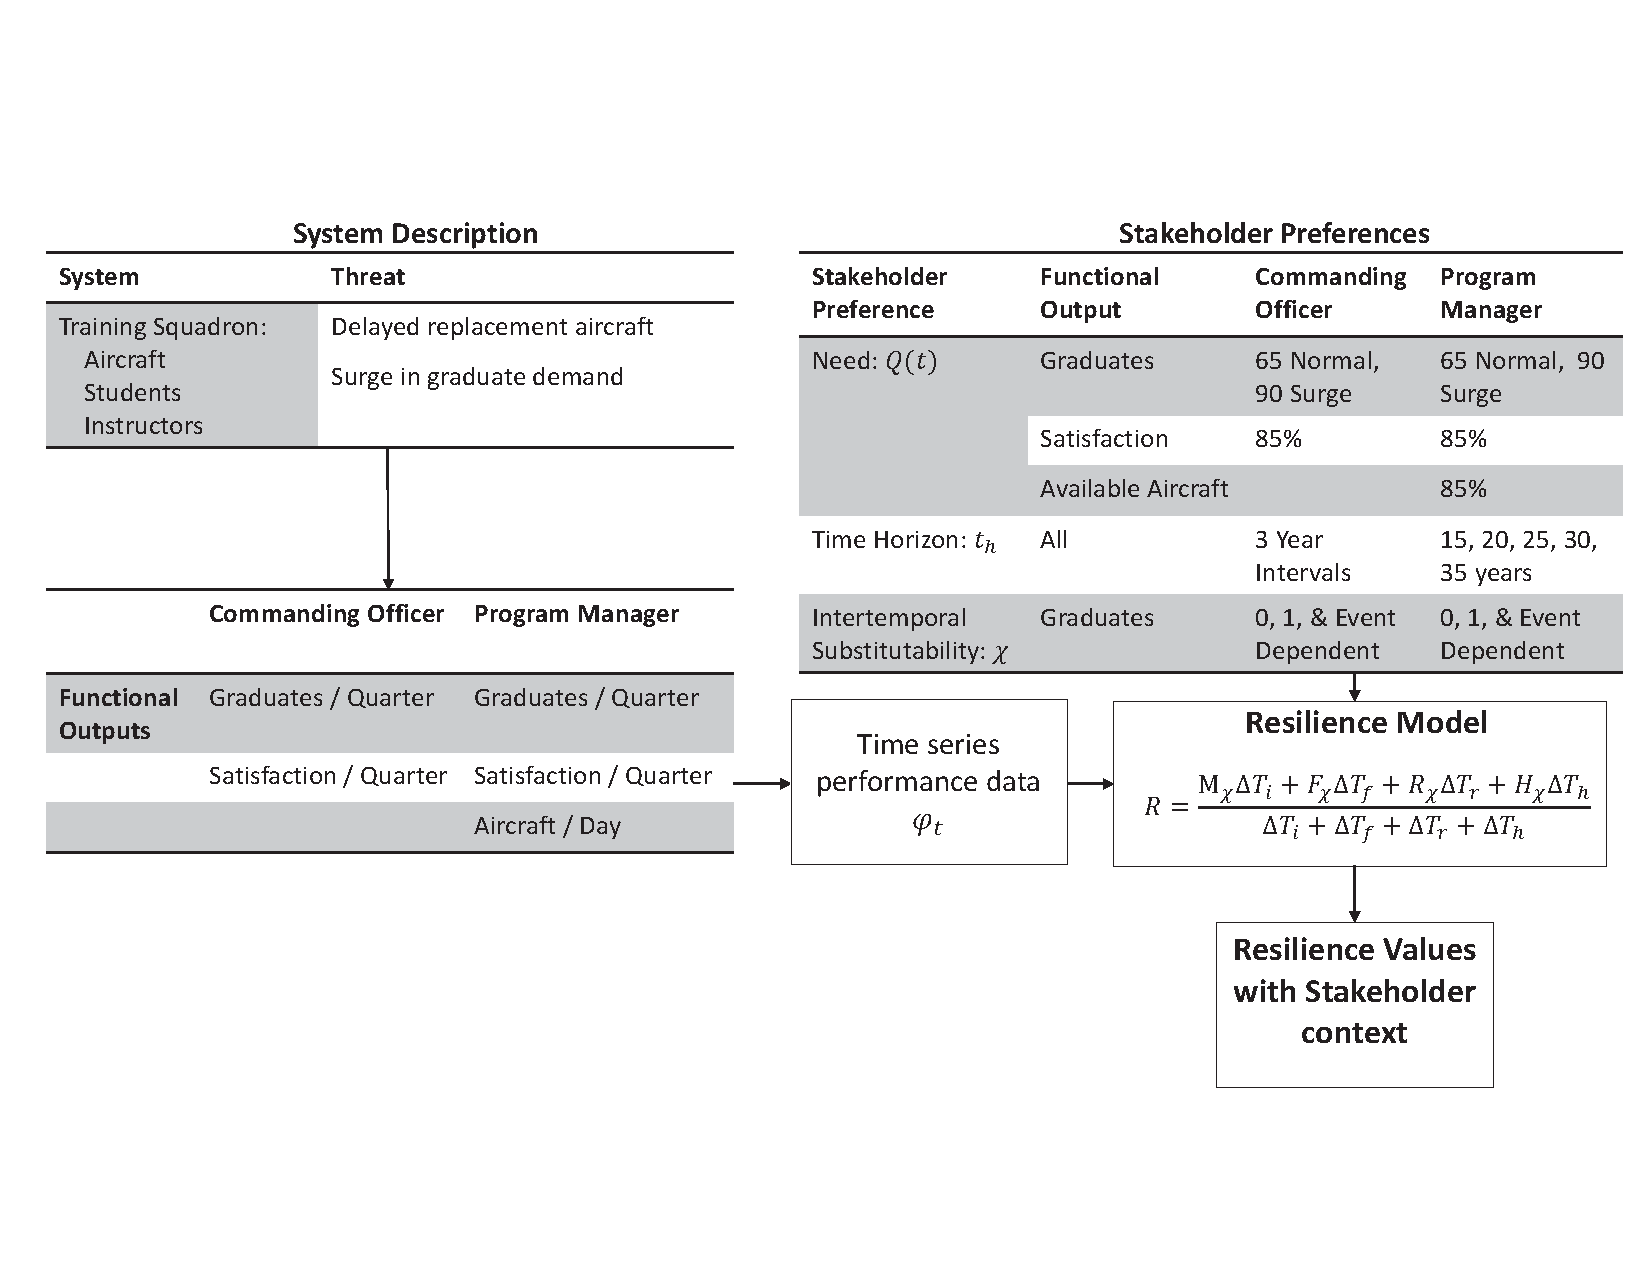
\includegraphics[width=\textwidth]{FleetHybridModelDetailedEmb}
  \caption{Case Study Hybrid Resilience Framework}
  \label{f:FleetFramework}
\end{figure}


\subsection{Training Squadron Simulation}

The simulation uses the SimPy \cite{Scherfke2018} package in Anaconda
Python 3.5 \cite{Anaconda2016}. SimPy contains 
prebuilt capability to define a simulation environment, processes, and
resources. The squadron simulation comprises two primary objects: aircrew and
aircraft. Multiple processes, defined by a scheduler object, determine
which aircraft and aircrew are available at a given time, and match
the available aircraft and aircrew to conduct a training event.

Figure~\ref{f:DESflow} depicts the simulation flow. The simulation
revolves around the event of a flight.  A flight requires a student,
an instructor, and an aircraft. At the completion of the flight, each
component of the aircraft is either up or down. If a component is
down, maintenance personnel repair the aircraft to return it to the
aircraft bin. Each component's expended life is compared to the
available life. Instructors grade students after each flight. The
grade is pass/fail. After a certain number of passing flights, the
student graduates and is placed in the graduate pool for assignment to
a tactical, as opposed to training, squadron.

The scenarios define the different possibilities for system behavior
and threats to the system under consideration. The system is a fleet
of 50 aircraft with a monthly matriculation of
25 students. Matriculation numbers are drawn from a uniform
distribution from 18 to 32.  The aircraft lifetime is 7,200 hours. Under this
\emph{normal} operating procedure, the  
aircraft last just to the planned end of life, or fifteen years.

The motivating problem is a change in sundown date. Much to the
chagrin of the program manager, the procurement of a follow-on
training aircraft has been delayed. To solve this problem the program manager
initiates a service life extension plan for the airframe. As each
aircraft approaches is life limit, it is placed in a queue to receive
modifications to enhance the lifetime. The study looks at extending
operational use of the fleet in five year increments from 15 years
(original lifetime) to 35 years.

The following sections define the simulation entities in more detail.

\begin{table}[h]
    \centering
    \begin{tabular}{l c }
      \hline
      \hline
      \textbf{Parameter} & \textbf{Value} \\
      \hline
      Aircraft & 50 \\
      Students & 50 \\
      Instructors & 40 \\
      Aircraft Lifetime & 7,200 Hours \\
      Aircraft SLEP trigger & 7,000 Hours \\
      \hline
    \end{tabular}
    \caption{Simulation Paramager Starting Values }
  \label{t:StartingValues}
\end{table}

\subsubsection{Aircraft Model}
An aircraft comprises three parts: airframe, avionics, and
propulsion. A part has a lifetime, a repair time, a failure rate. Part
failure rates are dependent only upon flight hours. In the simulation,
the failure distribution is an exponential distribution with $\lambda$
set as depicted in Table~\ref{t:PartSettings}. Parts repair is
as good as new, and the time to repair distribution is defined as a
log-normal distribution that remains the same throughout time. Further
studies could capture the uncertainty of these parameters and their
time/use dependence. The focus of this study is the intertemporal
substitutability factor and the discrete calculation of resilience, so
that will wait for another time.

Each part subclass, airframe, avionics, and propulsion has its own
failure distribution, repair distribution, SLEP trigger time,
lifetime, and lifetime added through SLEP. For this study, the
airframe is the part of primary significance. For  this case study,
only the airframe underwent SLEP. As a consequence, the airframe has
additional parameters of time to SLEP, additional  hours due to SLEP,
and age to start SLEP.

\begin{table}[h]
  \centering
  \begin{tabular}{l c c}
    \hline
    \hline
    \textbf{Part} & \textbf{Characteristic} & \textbf{Value (Hours)} \\
    \hline
    Airframe & \makecell{ Average Time to Failure \\ Average Time to
      Repair \\ Fatigue Life to Trigger SLEP}  &
    \makecell{ 100 \\ 720 \\ 7000} \\
    \hline
    Propulsion & \makecell{ Average Time to Failure \\ Average Time to
      Repair}  &
    \makecell{ 40 \\ 240 \\ } \\
    \hline
    Avionics & \makecell{ Average Time to Failure \\ Average Time to
      Repair}  &
    \makecell{ 30 \\ 240 \\ } \\
    \hline
  \end{tabular}
  \caption{Aircraft Simulation Values}
  \label{t:PartSettings}
\end{table}



\subsubsection{Aircrew}

Students and instructors are aircrew. Both
students and instructors record hours flown for the aircrew.  A
student graduates from the curriculum with 61 complete flights and
less than 4 failed 
flights \cite{Air2009}. The student enters the ``graduated students''
pool when the curriculum is complete. The student enters the
``attrited students'' pool after failing four flights. Each flight has
a 3.5\% chance to result in a failure. Over the course of 61 graded
flights, a student has an ~84 \% chance to graduate the syllabus. If a
part on the aircraft fails during the flight, the 
flight is graded as an incomplete, and must be re-flown. A student may
fly up to two flights per day. The simulation begins with a set
amount of students. Every 30 days new class of students
matriculates into the flight program. Table~\ref{t:aircrewParams}
summarizes the above parameters used for the students. The class size
can be manipulated to reflect the changing needs of the squadron
commander stakeholder and for sundown of the system. Instructors are
not a key part of this study. They may fly three flights a
day. For the purposes of this study instructors are controlled

\begin{table}[h]
  \centering
  \begin{tabular}{l c c}
    \hline
    \hline
    \textbf{Parameter} & \textbf{Student Value} & \textbf{Instructor Value} \\
    \hline
    Events per Day & 2 & 3 \\
    Events in Curriculum & 61 & NA \\
    Event Failure Rate & 3.5\% & NA \\
    Failed Events Allowed & 3 & NA \\
    \hline
  \end{tabular}
  \caption{Model Parameter Values for Students and Instructors}
  \label{t:aircrewParams}
\end{table}

Two other entities are important to the model, but in this study are
not stakeholders. The instructor aircrew  add
constraints to the model. One entity is the pool of
instructors. Instructors must be trained like students, albeit with a
shorter syllabus, and rotate out of the model at three year
intervals. Instructors constrain the number of students that can be
trained. The maintenance personnel pool constrains the number of
aircraft components that can be maintained.

\subsubsection{SLEP Simulation}

The program manager faces three different SLEP strategies: ``No
SLEP'', ``Small SLEP,'' and ``Large SLEP.'' ``As-Is'' does not add any
life to the aircraft, but it also avoids 
taking aircraft out of the flight schedule for the extended time
required to conduct SLEP. ``Small SLEP'' increases the 
lifetime of the aircraft to 14,400 flight hours, 
but the aircraft will be unavailable for 9 months during the
SLEP. ``Large SLEP'' increases the lifetime of the
aircraft to 18,000 flight hours, but the aircraft will be unavailable for
12 months during the SLEP.

An aircraft enters the SLEP line when it reaches its SLEP flight hour
limit. The SLEP line has a limited number of slots available in the
hangar, so the program manager gradually introduces aircraft to the
SLEP line. The simulation assigns each aircraft instantiation a SLEP
flight limit ranging from 3,500  to 7,000 flight hours to prevent
excessive wait times.  

\subsubsection{Flight Scheduling}
The scheduler is the heartbeat of the system. The scheduler uses a
simplified calendar with a five-day flying week and two day weekend
with maintenance but no flying. Each working (flying) day is split into 4
events spaced by 3 hours for each start time. The scheduler uses a
uniform distribution to select a flight time between 0.5 and 2.0 hours
for a single event.

The two disruptive events
are fleet wear-out and change in demand for graduates. Each flight
consumes a portion of the acceptable lifetime of each aircraft
component. When an aircraft's lifetime is exhausted, it must be
retired or undergo a life extension program. The alternative courses
of action are different options to extend the life of the
aircraft. Life extension activities remove aircraft from use to train
the flight line for life extension are unavailable for flights. While
fleet wear-out is a gradual, predictable event, demand for students
can fluctuate instantaneously.  The commanding officer must change the
daily flight schedule to accommodate these changes.


The scheduler assesses the available aircraft, instructors,
and students to make a match for the. Aircraft that have surpassed their SLEP flight hours are
sent to the SLEP line.  Aircraft in the SLEP line wait for an
SLEP spot to become available. Once an aircraft is in a SLEP spot, it
returns to the flight line after six or nine months, depending on the life
added to the system.  When aircraft that have surpassed their lifetime
they are no longer available for SLEP
or the flight schedule. For each event, the scheduler makes
student-instructor-aircraft matches for each event until one of the
pools is exhausted. The results of a flight are:
\begin{itemize}
\item Student outcomes:
  \begin{itemize}
  \item Flight incomplete due to aircraft failure
  \item Passing flight  for the student
  \item Failure of curriculum hop for the student
  \end{itemize}
\item Aircraft outcomes:
  \begin{itemize}
  \item Down status
  \item Up status
  \item Send to SLEP line
  \item End of life
  \end{itemize}
\end{itemize}

The scheduler updates all the objects involved in the flight: adds
flight hours added to the aircraft and parts; updates student syllabus
completion data; assesses student status (graduate, attrite,
continue); adds a new class of students monthly; assesses aircraft
repair status (up or down); assesses aircraft flightline status
(flightline, SLEP line, end of life); and assesses status of aircraft in
the SLEP line (waiting, in-SLEP, complete). 







%% \begin{table}[h]
%%   \resizebox{\textwidth}{!}{%
%%     \centering
%%     \begin{tabular}{l c c}
%%       \hline
%%       \hline
%%       \textbf{Course of Action} & \textbf{post-SLEP Lifetime} & \textbf{Time
%%         To SLEP (months)} \\
%%       \hline
%%       As-Is & NA (7,200) & NA  \\
%%       Small SLEP & 14,400 & 6 \\
%%       Large SLEP & 18,000 & 9 \\
%%       \hline
%%       \hline
%%     \end{tabular}}
%%     \caption{SLEP Courses of action}
%%   \label{t:SimScen}
%% \end{table}




\begin{figure}[h]
  \centering\includegraphics{DESflow.png}
  \caption{Squadron Fleet Operation Flow of Events}
  \label{f:DESflow}
\end{figure}



\subsection{Stakeholder Profiles}

The study comprises two stakeholder profiles: squadron
commanders and the program manager. Table~\ref{t:StakeholderPreferences}
shows the functional outputs of interest and the associated values for
time horizon, endogenous preference, and intertemporal
substitutability for each stakeholder.

The program manager is responsible for maintaining the
viability of the fleet of aircraft until a replacement system is
operational. Viability is assessed daily as the fraction of 
aircraft ready to provide training events to the total number of aircraft
assigned to the squadron. The program manager must also ensure the flight system
produces enough graduates over its lifetime and that time to train is
reasonable. The program manager's time horizon is uncertain. The
resilience analytical model outputs values at 15, 20, 25, 30, and 35
years of aircraft operations.  

The commanding officer has two functional outputs of interest:
graduates per quarter and satisfaction rate. The
percentage of students graduating under the time limit per quarter is
the satisfaction rate. Squadron Commanders have a three-year
tenure which is their time horizon $t_h$. Although, in reality,
Squadron Commanders are conscientious 
individuals, the simulation treats them as singularly focused upon
their period of command with no concern of quota satisfaction before
or after them. A surplus of graduates during one quarter may have value
transferable to the previous or following quarter. The study will
investigate different types of intertemporal substitutability to include
\emph{ephemeral}, \emph{permanent}, and \emph{adjacent}
values. Graduate satisfaction rates are \emph{ephemeral} ($\chi = 0$).


\subsection{Study Scenarios}

The study has two main thrusts of inquiry. One goal is to demonstrate
the hybrid resilience framework in the domain of a fleet of systems
satisfying multiple stakeholders with multiple preference
profiles. Another goal is to demonstrate the \emph{adjacent}
intertemporal substitutability algorithm.

\subsubsection{Hybrid Resilience Framework Demonstration}

The previous sections discussed the system, simulation, and resilience
analytical framework. The program manager has three courses of action
for supporting the aircraft (Table~\ref{t:SimScen}): do nothing
(``As-Is''), increase the operational life to 14,400 flight hours
(``Small SLEP''), or increase the operational life to 18,000 flight
hours (``Large SLEP''). The program manager must also consider a
change in demand for graduates. This study investigates the impact of
a two year ``surge'' of desired graduates manifested by larger
incoming classes and an increase in endogenous need. The average class
size increases to 35 per month from a normal size of 25. A uniform
distribution for 70-130\% of the average class size 
provides variation in the class size per month. The demand
for students increases from 65 students per quarter to 90 students per
quarter. 

\begin{table}[h]
  \resizebox{\textwidth}{!}{%
    \centering
    \begin{tabular}{l c c}
      \hline
      \hline
      \textbf{Course of Action} & \textbf{post-SLEP Lifetime} & \textbf{Time
        To SLEP (months)} \\
      \hline
      As-Is & NA (7,200) & NA  \\
      Small SLEP & 14,400 & 6 \\
      Large SLEP & 18,000 & 9 \\
      \hline
      \hline
    \end{tabular}}
    \caption{SLEP Courses of Action}
  \label{t:SimScen}
\end{table}

\begin{table}[h]
    \centering
    \begin{tabular}{l c c c}
      \hline
      \hline
      \textbf{Operations} & \makecell{\textbf{Minimum Class} \\ (month)} &
      \makecell{\textbf{Maximum Class} \\ (month)} & \makecell{\textbf{Desired Graduates} \\ (quarter)}\\
      \hline
      Normal  & 18 & 32 & 65\\
      Surge  & 25 & 41 & 90\\
      \hline
    \end{tabular}
    \caption{Student Class Sizes}
  \label{t:StudScen}
\end{table}


\begin{table}[h]
  \resizebox{\textwidth}{!} 
    % based on\\ demands for students} 
    & \makecell{Ephemeral, Permanent, Adjacent \\ Ephemeral} \\
    \hline
    \makecell[c]{Program \\ Manager}    & \makecell[c]{Daily Availability \\ Quarterly
      Graduates \\ Student Satisfaction} & {15-35 Years} &
    \makecell[c]{85\% \\ Normal (65) / Surge (90) \\ 85\%} 
      % based upon \\ usage by
      %Commanding Officer} 
      & \makecell[c]{Ephemeral \\ Ephemeral, Permanent, Adjacent \\ Ephemeral} 
      \\
    \hline
  \end{tabular}}
  \caption{Stakeholder Preference Profile}
  \label{t:StakeholderPreferences}
\end{table}


\subsubsection{Intertemporal Substitutability Investigation}

The study conducted an exploration of intertemporal substitutability
values applied to the algorithm described above. This is applicable to
the graduates per quarter functional output. Simulation data
post-processing applied 12 different values for $\chi$ to graduates
per quarter. The values for $\chi$ adjusted the amount of time steps
that had value, the coefficient of the value, and whether surplus
before and after had an impact. Table~\ref{t:StakeholderChiPreferences} shows the
values used. Negative time steps are time steps before the shortfall
while positive time steps  are after the shortfall. 

\begin{table}[h]
  \centering
  \begin{tabular}{l c c c c c c c c}
    \hline
    \hline
    & \multicolumn{8}{c}{\textbf{Index ($j$)}}\\\cline{2-9}
    \textbf{Case} &
    \textbf{-4} &
    \textbf{-3} &
    \textbf{-2} &
    \textbf{-1} &
    \textbf{1} &
    \textbf{2} &
    \textbf{3} &
    \textbf{4}\\
    \hline
    %%     &   -4 &   -3 &   -2 &   -1 &    1 &    2 &    3 &    4 \\
    \multicolumn{9}{l}{Substitute only \emph{after} shortfall} \\
    A1 &    0 &    0 &    0 &    0 &  0.5 &    0 &    0 &    0 \\                       
    A2 &    0 &    0 &    0 &    0 &  0.5 & 0.25 &    0 &    0 \\                       
    A3 &    0 &    0 &    0 &    0 &    1 &  0.5 &    0 &    0 \\
    A4 &    0 &    0 &    0 &    0 &    1 &    1 &    1 &    1\ldots \\
    \multicolumn{9}{l}{Substitute only \emph{before} shortfall} \\
    B1 &    0 &    0 &    0 &  0.5 &    0 &    0 &    0 &    0 \\                       
    B2 &    0 &    0 & 0.25 &  0.5 &    0 &    0 &    0 &    0 \\                       
    B3 &    0 &    0 &  0.5 &    1 &    0 &    0 &    0 &    0 \\
    B4 & \ldots1 & 1 &    1 &    1 &    0 &    0 &    0 &    0 \\
    \multicolumn{9}{l}{Substitute \emph{before} \& \emph{after} shortfall} \\
    C1 &    0 &    0 &    0 &  0.5 &  0.5 &    0 &    0 &    0 \\                       
    C2 &    0 &    0 &  0.5 &    1 &    1 &  0.5 &    0 &    0 \\                       
    C3 &    0 &    0 & 0.25 &  0.5 &  0.5 & 0.25 &    0 &    0 \\                       
    C4 & 0.25 &  0.5 & 0.75 &    1 &    1 & 0.75 &  0.5 & 0.25 \\                       
    Ephemeral &  0 &  0 &    0 &  0 &    0 &    0 &    0 &    0 \\                       
    Permanent & \ldots 1 &  1 &    1 &  1 &    1 &    1 &    1 &
    1\ldots \\
    \hline
    \end{tabular}
  \caption{Values for $\chi$ Matrices}
  \label{t:StakeholderChiPreferences}
\end{table}


\section{Results}
\label{s:Results}
%% \subsection{Simulation Execution}

%% A parameter file provided the simulation the key inputs: SLEP type,
%% surge status, and number of runs per scenario. Each simulation run
%% takes 3-15 minutes, so multiple machines ran the simulation. The
%% simulation defined a random seed at the beginning of each
%% experiment. The simulation reset the seed at the beginning of each new
%% scenario to ensure a replicated draw between the experiments. Each
%% experiment comprised 5,275 runs.


\subsection{Simulation Outputs}

The discrete event simulation produces time-series data for aircraft
disposition and status status; graduates, attrites, and matriculated
students; and time to graduate for each
student. Figures~\ref{f:ts_no_surge} shows an example run for the ``No
surge'' scenarios for each course of action. The solid line is the number of aircraft on the
flightline, the dashed line is the desired number of graduates per
quarter, and the points are the actual number of graduates in a
quarter. Figure ~\ref{f:ts_surge} shows the same information for the
``Surge'' scenario. The shaded area from 12-14 years highlights the
two year surge in required graduates.


\begin{figure}[h]
  \centering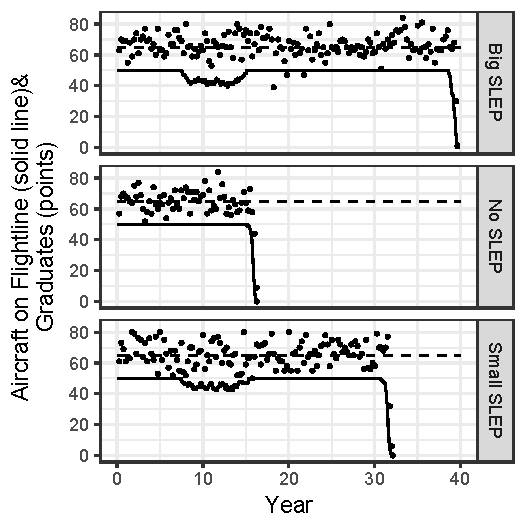
\includegraphics{time_series_fleet_no_surge}
  \caption{Simulation Output Example of Aircraft Data and Quarterly
    Graduates for each SLEP Option without Surge in Students}
  \label{f:ts_no_surge}
\end{figure}

\begin{figure}[h]
  \centering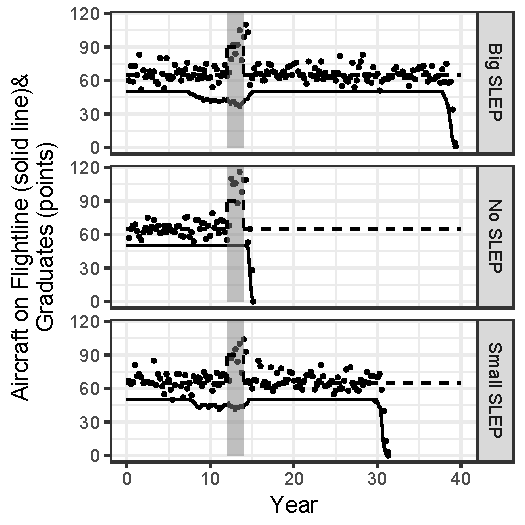
\includegraphics{time_series_fleet_surge}
  \caption{Simulation Output Example of Aircraft Data and Quarterly
    Graduates for each SLEP Option without Surge in Students}
  \label{f:ts_surge}
\end{figure}



\subsubsection{Resilience Results}

The configuration of the boxplots show the maximum, minimum and
quartiles of the resilience values. The ends of the vertical lines are
the maximum and minimum resilience; the top and bottom edges  of the box are the
75th and 25th percentiles; and the dark hash is the median resilience.

\subsection{Program Managers}

The Program Manager applies the preference profiles and desired
functional outputs defined in
Table~\ref{t:StakeholderPreferences}. A series of three figures presents
the program manager resilience results. Each figure shows the results
for a single time horizon. This presentation enables visual inspection
of the preferred course of action.  The Figures~\ref{f:PMresultsAo15},
\ref{f:PMresultsAo25}, and \ref{f:PMresultsAo35} show results for
the daily aircraft ready to fly functional
output. Figures~\ref{f:PMresultsGrad15},
\ref{f:PMresultsGrad25}, and \ref{f:PMresultsGrad35} show results for
the graduates per quarter output for \emph{ephemeral} and
\emph{permanent} values of $\chi$. Figures~\ref{f:PMresultsSat15},
\ref{f:PMresultsSat25}, and \ref{f:PMresultsSat35} show results for
the student satisfaction functional output. Table~\ref{t:PreferredCOA_PM_No_Chi} shows the program
manager's preferred course of action for each 
functional outputs' resilience at each time horizon. In the table,
``Adjacent'' refers to case C4.
\begin{figure}[h]
  \centering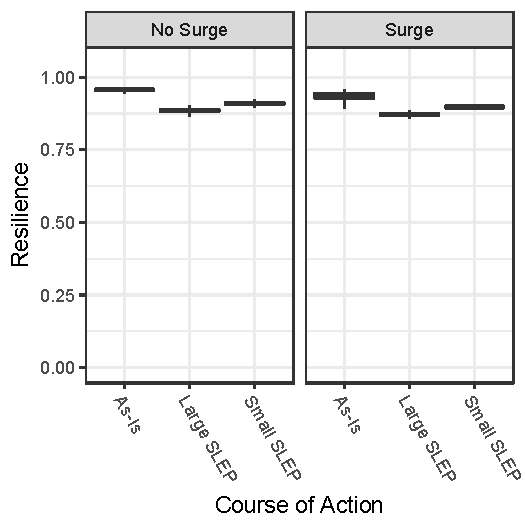
\includegraphics{PMAoPlotTimeHorizon15}
  \caption{Program Manager Daily Ready Aircraft Resilience Results - 15 Year Time Horizon}
  \label{f:PMresultsAo15}
\end{figure}

\begin{figure}[h]
  \centering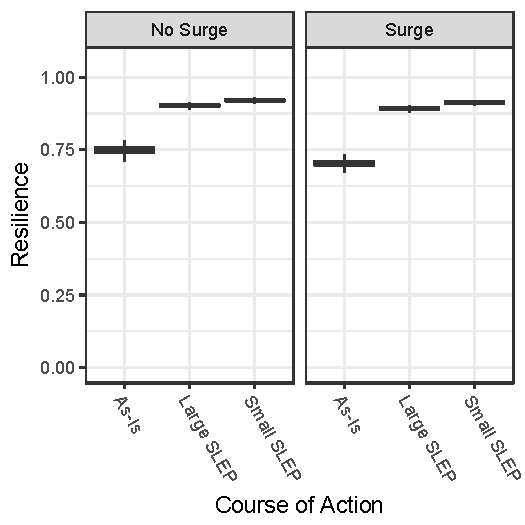
\includegraphics{PMAoPlotTimeHorizon20}
  \caption{Program Manager Daily Ready Aircraft Resilience Results - 15 Year Time Horizon}
  \label{f:PMresultsAo20}
\end{figure}

\begin{figure}[h]
  \centering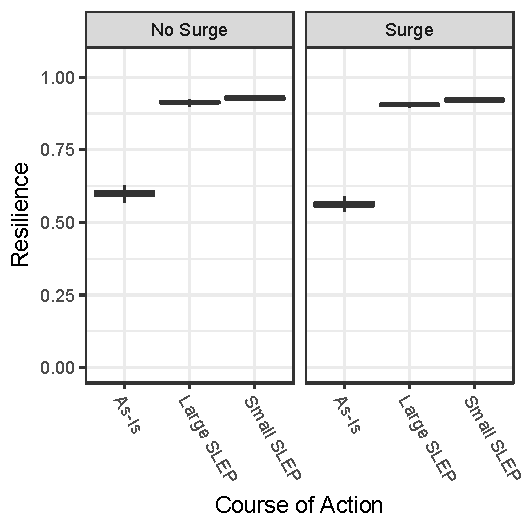
\includegraphics{PMAoPlotTimeHorizon25}
  \caption{Program Manager Daily Ready Aircraft Resilience Results - 25 Year Time Horizon}
  \label{f:PMresultsAo25}
\end{figure}

\begin{figure}[h]
  \centering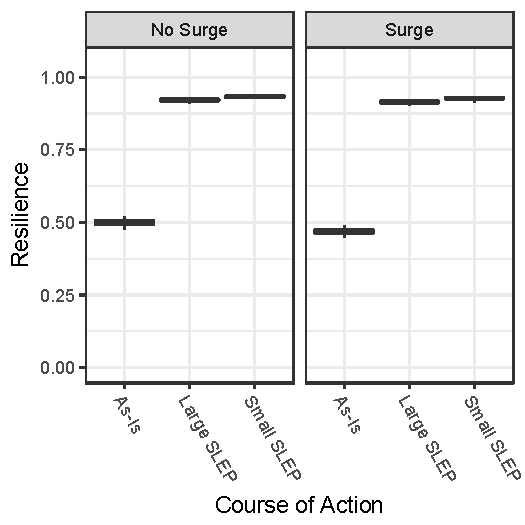
\includegraphics{PMAoPlotTimeHorizon30}
  \caption{Program Manager Daily Ready Aircraft Resilience Results - 15 Year Time Horizon}
  \label{f:PMresultsAo30}
\end{figure}

\begin{figure}[h]
  \centering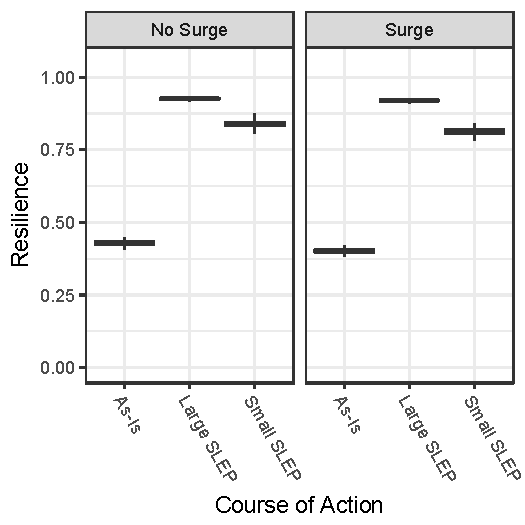
\includegraphics{PMAoPlotTimeHorizon35}
  \caption{Program Manager Daily Ready Aircraft Resilience Results - 35 Year Time Horizon}
  \label{f:PMresultsAo35}
\end{figure}


\begin{figure}[h]
  \centering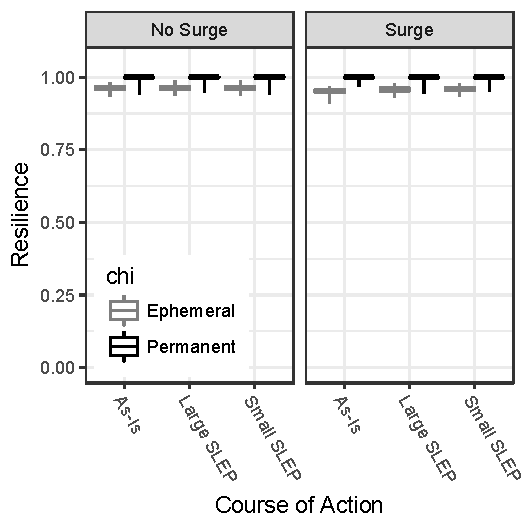
\includegraphics{PMGradPlotTimeHorizon15}
  \caption{Program Manager Graduates per Quarter Resilience Results - 15 Year Time Horizon - 15 Year Time Horizon}
  \label{f:PMresultsGrad15}
\end{figure}

\begin{figure}[h]
  \centering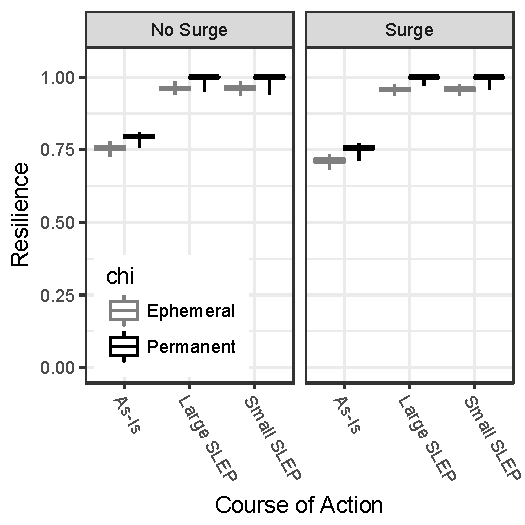
\includegraphics{PMGradPlotTimeHorizon20}
  \caption{Program Manager Graduates per Quarter Resilience Results - 15 Year Time Horizon - 15 Year Time Horizon}
  \label{f:PMresultsGrad20}
\end{figure}


\begin{figure}[h]
  \centering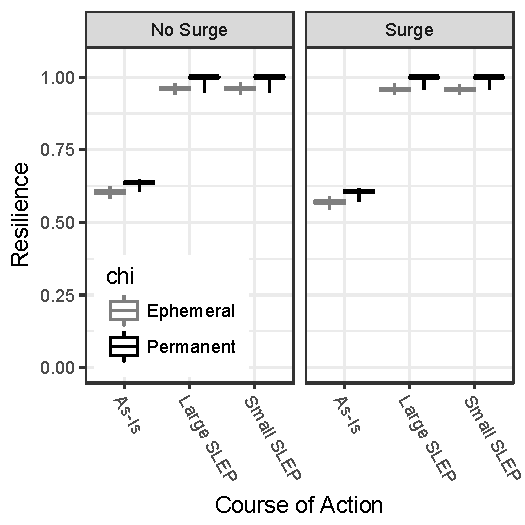
\includegraphics{PMGradPlotTimeHorizon25}
  \caption{Program Manager Graduates per Quarter Resilience Results - 25 Year Time Horizon}
  \label{f:PMresultsGrad25}
\end{figure}

\begin{figure}[h]
  \centering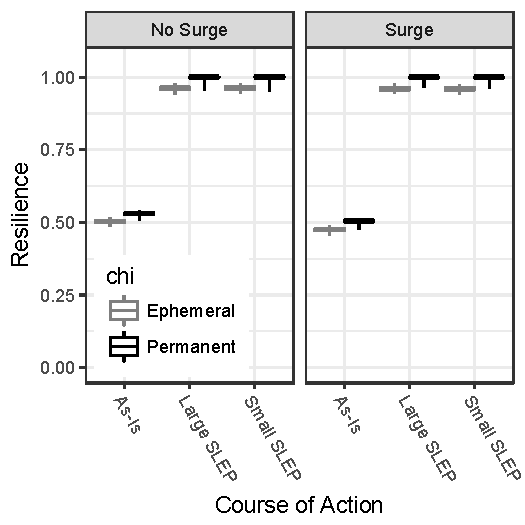
\includegraphics{PMGradPlotTimeHorizon30}
  \caption{Program Manager Graduates per Quarter Resilience Results - 15 Year Time Horizon - 15 Year Time Horizon}
  \label{f:PMresultsGrad30}
\end{figure}


\begin{figure}[h]
  \centering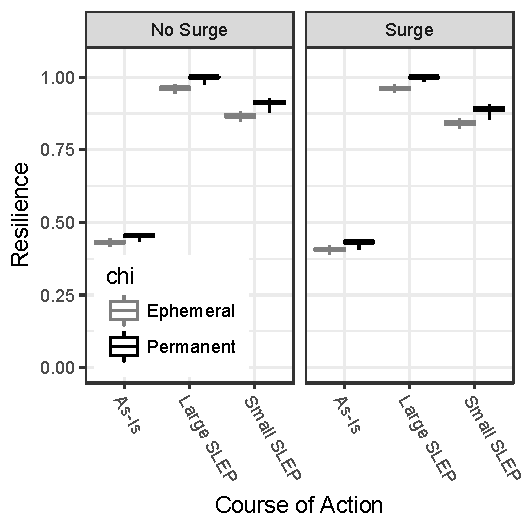
\includegraphics{PMGradPlotTimeHorizon35}
  \caption{Program Manager Graduates per Quarter Resilience Results - 35 Year Time Horizon}
  \label{f:PMresultsGrad35}
\end{figure}

\begin{figure}[h]
  \centering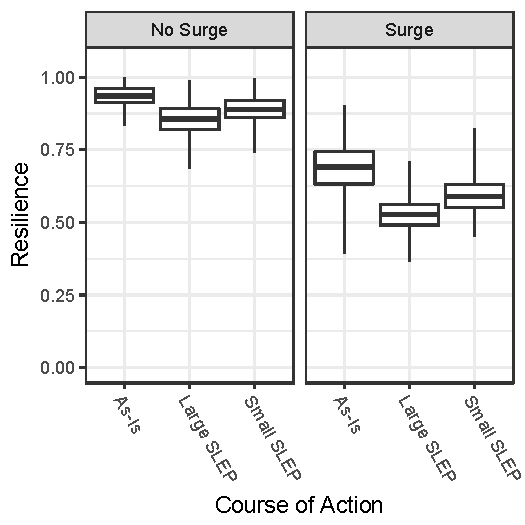
\includegraphics{PMSatPlotTimeHorizon15}
  \caption{Program Manager Student Satisfaction Resilience Results - 15 Year Time Horizon}
  \label{f:PMresultsSat15}
\end{figure}

\begin{figure}[h]
  \centering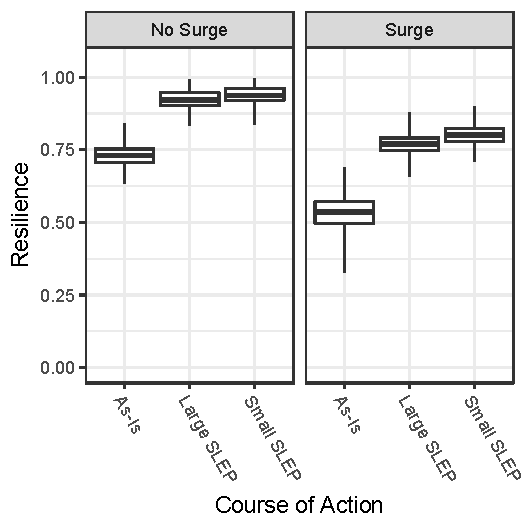
\includegraphics{PMSatPlotTimeHorizon20}
  \caption{Program Manager Student Satisfaction Resilience Results - 15 Year Time Horizon}
  \label{f:PMresultsSat20}
\end{figure}

\begin{figure}[h]
  \centering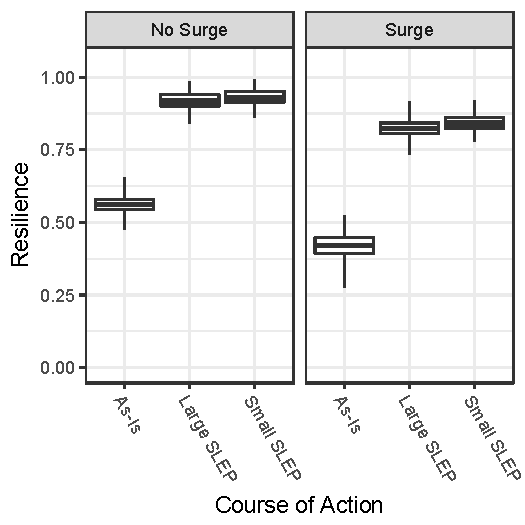
\includegraphics{PMSatPlotTimeHorizon25}
  \caption{Program Manager Student Satisfaction Resilience Results - 25 Year Time Horizon}
  \label{f:PMresultsSat25}
\end{figure}

\begin{figure}[h]
  \centering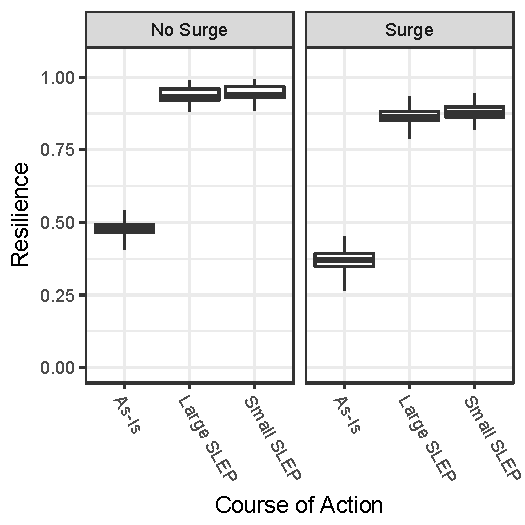
\includegraphics{PMSatPlotTimeHorizon30}
  \caption{Program Manager Student Satisfaction Resilience Results - 15 Year Time Horizon}
  \label{f:PMresultsSat30}
\end{figure}

\begin{figure}[h]
  \centering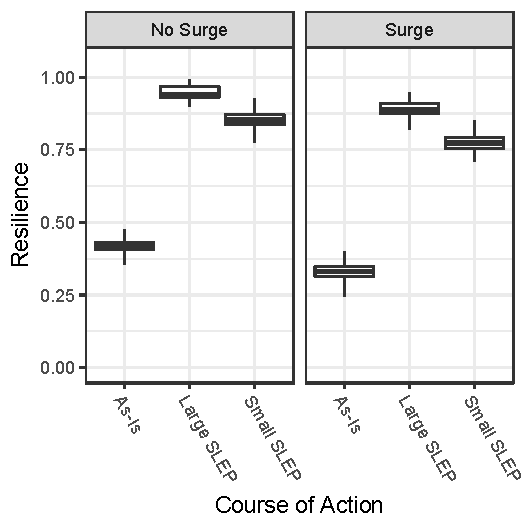
\includegraphics{PMSatPlotTimeHorizon35}
  \caption{Program Manager Student Satisfaction Resilience Results - 35 Year Time Horizon}
  \label{f:PMresultsSat35}
\end{figure}


\begin{table}[h]
  \centering
     \resizebox{\textwidth}{!}{%
\begin{tabular}{lcccccc}
  \hline
  \hline
  \multirow{2}{*}{\makecell{\textbf{Surge} \\ \textbf{Status}}} &
  \multirow{2}{*}{\makecell{\textbf{Time} \\ \textbf{Horizon}}} & 
  \multirow{2}{*}{\textbf{Availability}} &
  \multirow{2}{*}{\makecell{\textbf{Student}
      \\ \textbf{Satisfaction}}} &
  \multicolumn{3}{c}{\textbf{Grad}} \\\cline{5-7}
  & & & & \textbf{Ephemeral} & \textbf{Permanent}
  \\
  \hline
  \multirow{5}{*}{No Surge}
  %% Data comes from COandPMplots.R filfe Ao -> PMAoRating
  %% 
  & 15 & As-Is      & As-Is      & Small  &  All \\
  & 20 & Small  & Small  & Small  &  Large \& Small  \\
  & 25 & Small  & Small  & Small  &  Large \& Small \\
  & 30 & Small  & Small  & Small  &  Large \& Small  \\
  & 35 & Large  & Large  & Large  &  Large  \\
  \hline
  \multirow{5}{*}{Surge}
  & 15 & As-Is      & As-Is      & Small  &  Large \& Small  \\
  & 20 & Small  & Small  & Small  &  Large \& Small  \\
  & 25 & Small  & Small  & Small  &  Large \& Small  \\
  & 30 & Small  & Small  & Large  &  Large \& Small  \\
  & 35 & Large  & Large  & Large  &  Large  \\
  \hline
\end{tabular}}
  \caption{Program Manager Preferred Course of Action}
  \label{t:PreferredCOA_PM_No_Chi}
\end{table}

\subsection{Squadron Commanders}

The Squadron Commander applies the preference profiles and functional
outputs defined in Table~\ref{t:StakeholderPreferences}. Every
Squadron Commander has a three year time horizon. The squadron commanders are
identified alphabetically. Time periods with all aircraft life
expended have no commanding officers. Letters represent each
commanding officer. The first commanding officer was 
Commander Alpha (A). The ``As-Is'' course of action typically ends
with Commander Foxtrot (F); the ``Large SLEP'' course of action ends
with Commander November (N); and the ``Small SLEP'' course of action
usually ends with Commander Kilo (K), but occasionally reaches
Commander Lima. When a simulation runs out of aircraft, the Commander
receives no resilience value.

Figure~\ref{f:CO_Grad} shows the resilience
results for graduates per quarter for three intertemporal
substitutability values: the \emph{ephemeral} case, the
\emph{permanent} case and  \emph{adjacent} case C3
(Table~\ref{t:StakeholderChiPreferences}). Figure ~\ref{f:CO_Sat} shows the results for
resilience of satisfied graduates (less than 60 days in the squadron)
for each course of action and surge status. Figures~\ref{CO_D_Grad}
and \ref{CO_E_Grad}
\begin{figure}[h]
  \centering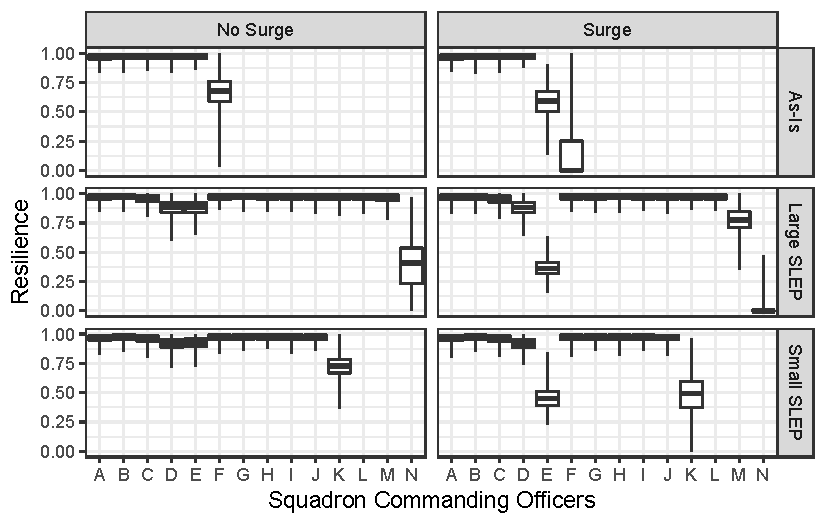
\includegraphics{CO_Sat}
  \caption{Squadron Commander Student Satisfaction Resilience Results}
  \label{f:CO_Sat}
\end{figure}

\begin{figure}[h]
  \centering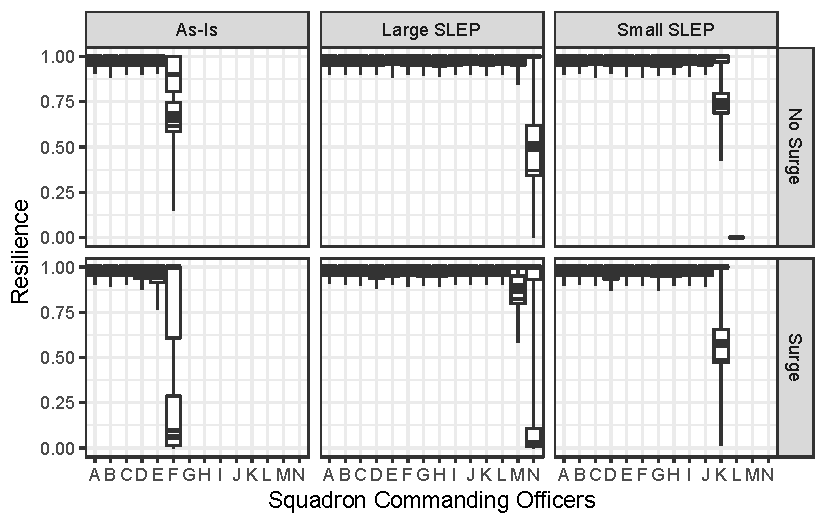
\includegraphics{CO_Grad}
  \caption{Squadron Commander Graduates per Quarter Resilience
    Results($\chi$ = 0)}
  \label{f:CO_Grad}
\end{figure}



%% \begin{table}[h]
%%   \centering
%%      \resizebox{\textwidth}{!}{%
%% \begin{tabular}{lccccc}
%%   \hline
%%   \hline
%%   \multirow{2}{*}{\makecell{\textbf{Surge} \\ \textbf{Status}}} &
%%   \multirow{2}{*}{\makecell{\textbf{Time} \\ \textbf{Horizon}}} & 
%%   \multirow{2}{*}{\makecell{\textbf{Student}
%%       \\ \textbf{Satisfaction}}} &
%%   \multicolumn{3}{c}{\textbf{Grad}} \\\cline{4-6}
%%   & & & \textbf{Ephemeral} & \textbf{Adjacent} & \textbf{Permanent}
%%   \\
%%   \hline
%%   \multirow{14}{*}{No Surge}
%%   %% Data comes from COandPMplots.R filfe Ao -> PMAoRating
%%   %% 
%%   & A & As-Is  & As-Is           & As-Is           & Large \\
%%   & B & Small  & Small           & Small           & Small \\
%%   & C & Large  & As-Is \& Large  & As-Is           & Large \\
%%   & D & As-Is  & Small           & Small           & All \\
%%   & E & Small  & All             & Small           & All \\
%%   & F & Large  & Large \& Small  & Large \& Small  & Large \& Small  \\
%%   & G & Large  & Large \& Small  & Large \& Small  & Large \& Small  \\
%%   & H & Large  & Large \& Small  & Large           & Large \& Small  \\
%%   & I & Large  & Large \& Small  & Small           & Large \& Small  \\
%%   & J & Large  & Large           & Large           & Large \& Small  \\
%%   & K & Large  & Large           & Large           & Large \& Small  \\
%%   & L & Large  & Large           & Large           & Large  \\
%%   & M & Large  & Large           & Large           & Large  \\
%%   & N & Large  & Large           & Large           & Large  \\
%%   \hline
%%   \multirow{14}{*}{Surge}
%%   %% Data comes from COandPMplots.R filfe Ao -> PMAoRating
%%   %% 
%%   & A & As-Is  & As-Is           & As-Is           & Large & Small \\
%%   & B & Small  & Large           & Small           & As-Is \\
%%   & C & Large  & As-Is           & Large           & Large \\
%%   & D & As-Is  & Small           & Small           & All \\
%%   & E & Small  & All             & Small           & All \\
%%   & F & Large  & Large \& Small  & Large \& Small  & Large \& Small  \\
%%   & G & Large  & Large \& Small  & Large \& Small  & Large \& Small  \\
%%   & H & Large  & Large \& Small  & Large           & Large \& Small  \\
%%   & I & Large  & Large \& Small  & Small           & Large \& Small  \\
%%   & J & Large  & Large           & Large           & Large \& Small  \\
%%   & K & Large  & Large           & Large           & Large \& Small  \\
%%   & L & Large  & Large           & Large           & Large  \\
%%   & M & Large  & Large           & Large           & Large  \\
%%   & N & Large  & Large           & Large           & Large  \\
%%    \hline
%% \end{tabular}}
%%   \caption{Commanding Officer Preferred Course of Action for each
%%     Functional Output Using Worst Case Scenario}
%%   \label{t:PreferredCOA_CO}
%% \end{table}

\subsection{Intertemporal Substitutability Investigation}

The second part of this study focused on implementing the
Intertemporal Substitutability algorithm. The study applied 12
\emph{adjacent} algorithms and the pre-existing \emph{permanent} and
\emph{ephemeral} cases. Intertemporal substitutability applied to the
graduates per quarter functional output of the
simulation. Figures~\ref{f:PMresultsGradAllChi15}, ~\ref{f:PMresultsGradAllChi20},
~\ref{f:PMresultsGradAllChi25}, ~\ref{f:PMresultsGradAllChi30}, and
~\ref{f:PMresultsGradAllChi35}  show the change in
resilience as the intertemporal substitutability changes for the
program manager.

\begin{figure}[h]
  \centering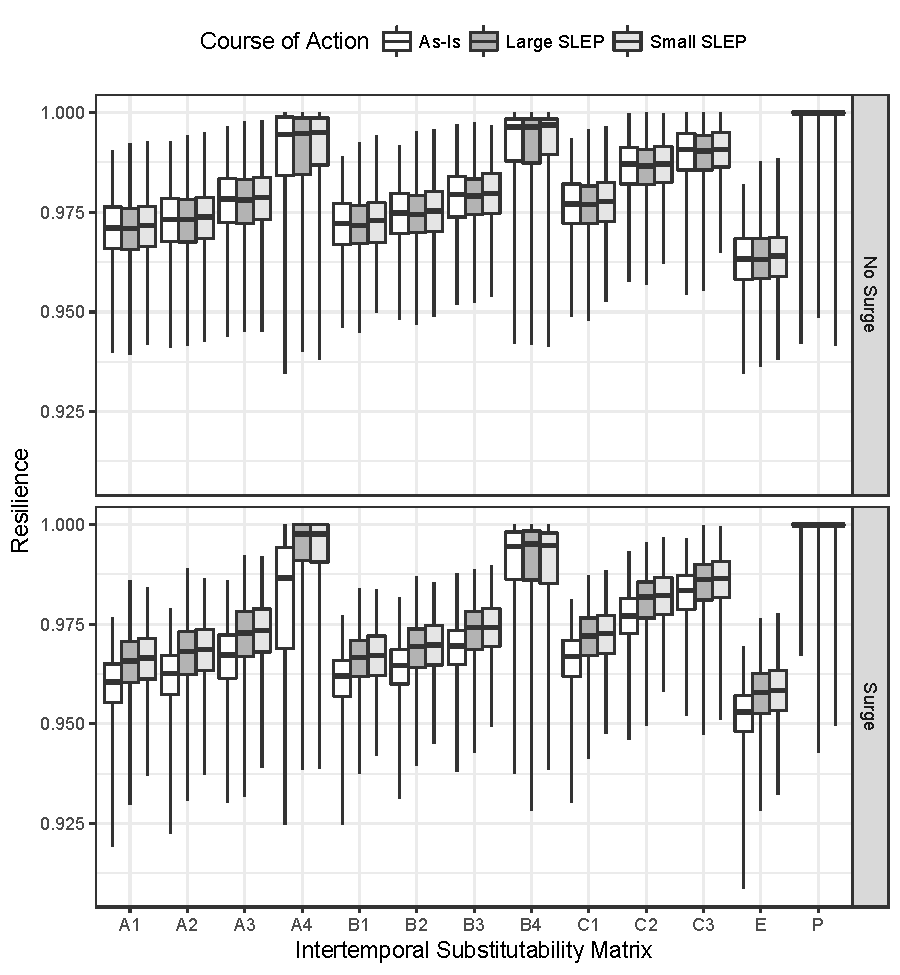
\includegraphics{PMGradAllChiPlotTimeHorizon15}
  \caption{Program Manager Graduates per Quarter Resilience Results  - 15 Year Time Horizon}
  \label{f:PMresultsGradAllChi15}
\end{figure}


\begin{figure}[h]
  \centering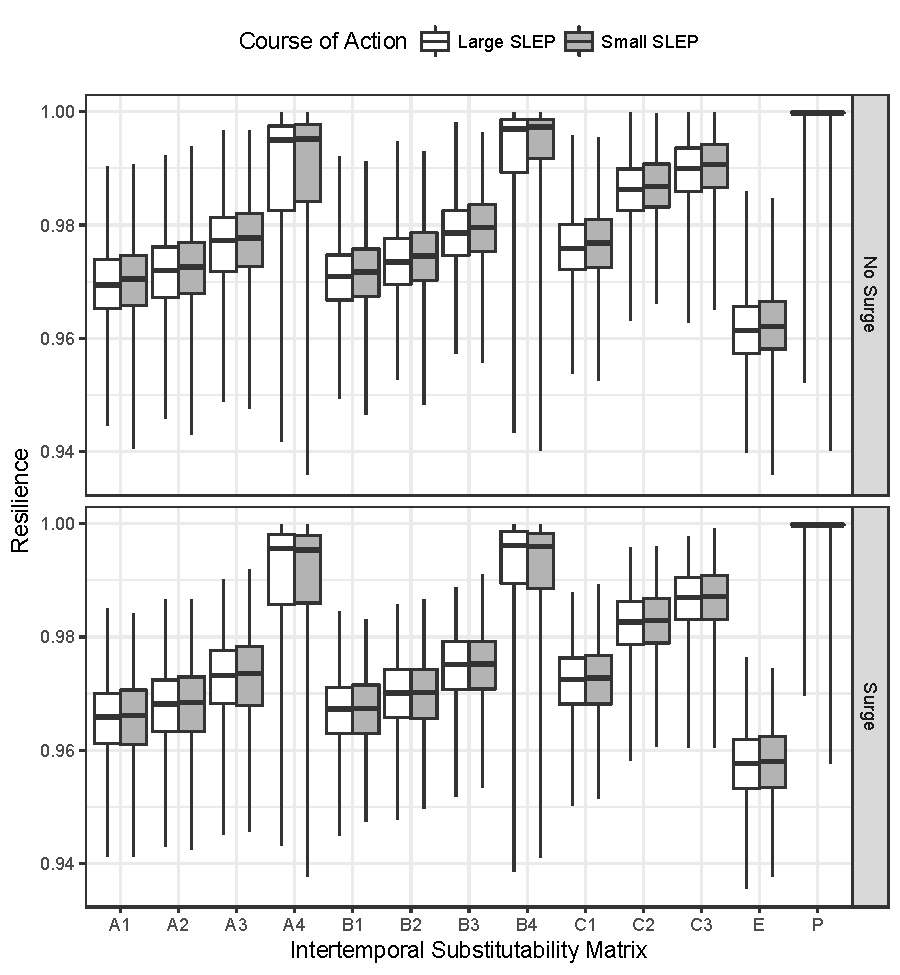
\includegraphics{PMGradAllChiPlotTimeHorizon20}
  \caption{Program Manager Graduates per Quarter Resilience Results  - 20 Year Time Horizon}
  \label{f:PMresultsGradAllChi20}
\end{figure}

\begin{figure}[h]
  \centering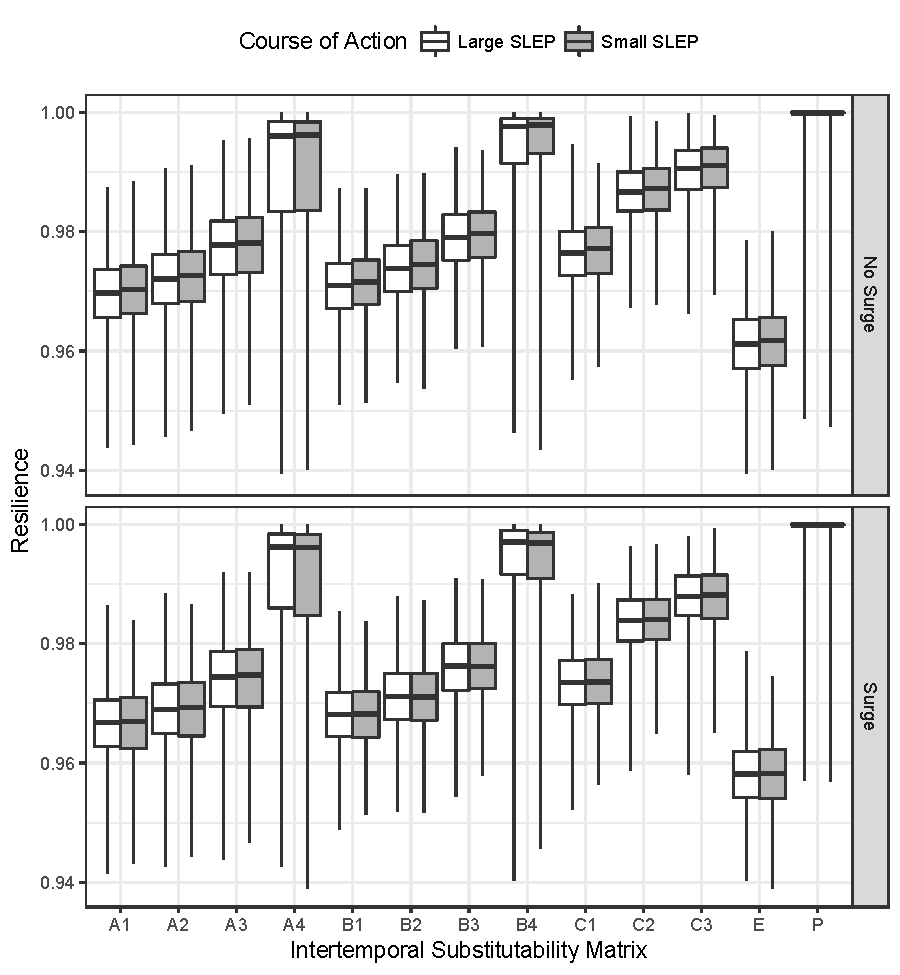
\includegraphics{PMGradAllChiPlotTimeHorizon25}
  \caption{Program Manager Graduates per Quarter Resilience Results - 25 Year Time Horizon}
  \label{f:PMresultsGradAllChi25}
\end{figure}

\begin{figure}[h]
  \centering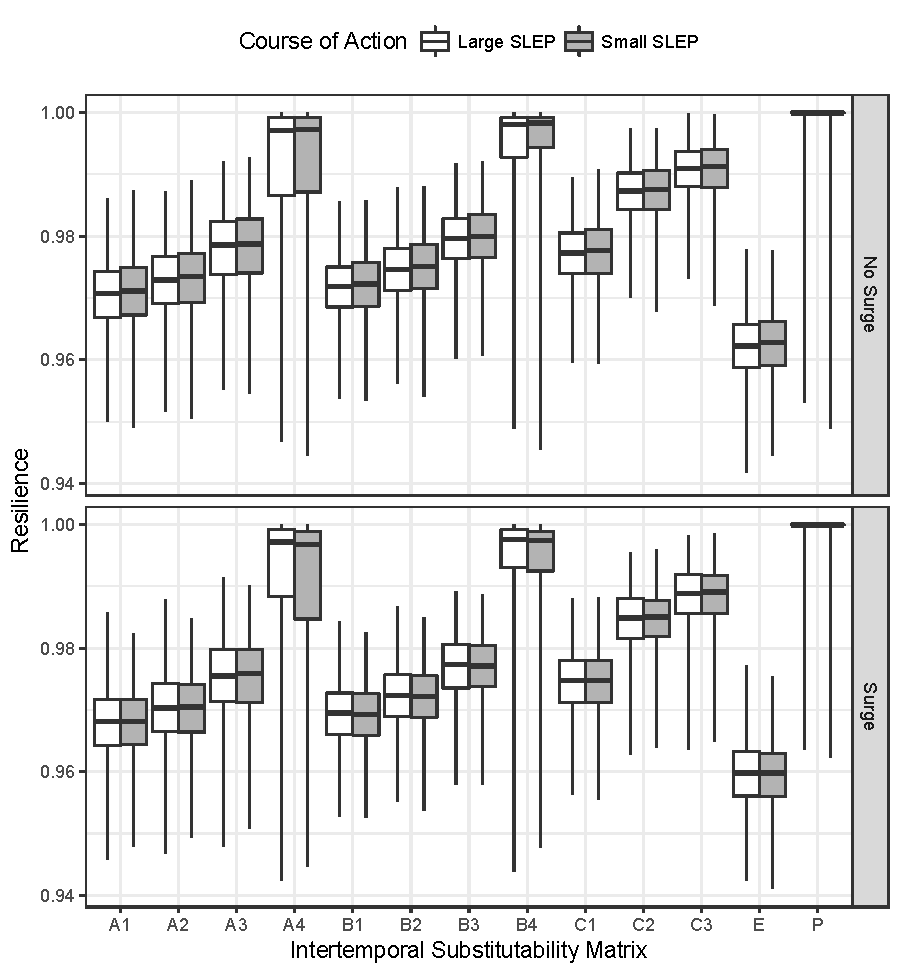
\includegraphics{PMGradAllChiPlotTimeHorizon30}
  \caption{Program Manager Graduates per Quarter Resilience Results  - 30 Year Time Horizon}
  \label{f:PMresultsGradAllChi30}
\end{figure}

\begin{figure}[h]
  \centering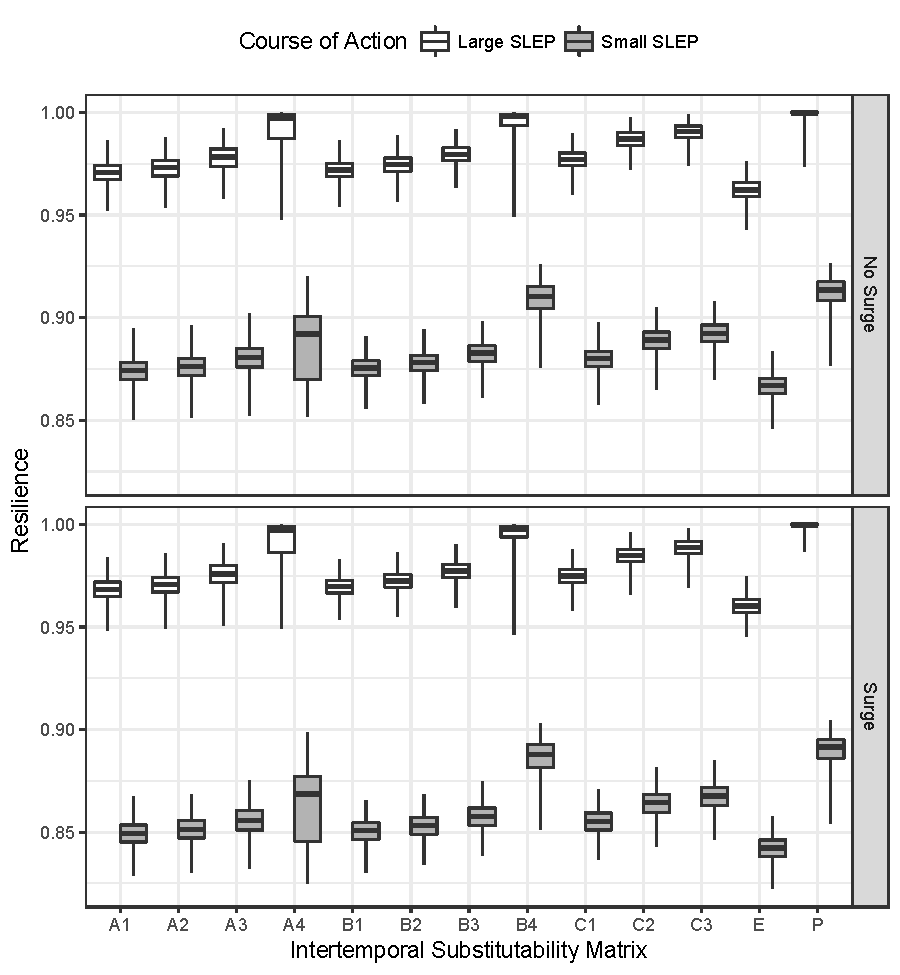
\includegraphics{PMGradAllChiPlotTimeHorizon35}
  \caption{Program Manager Graduates per Quarter Resilience Results - 35 Year Time Horizon}
  \label{f:PMresultsGradAllChi35}
\end{figure}

Figures~\ref{f:CO_D_Grad} and ~\ref{f:CO_E_Grad} show
the resilience values for all intertemporal substitutability
preferences from the perspective of Commanders Delta and 
Echo. The SLEP process and surge occur during these two commanders'
tenure.

\begin{figure}[h]
  \centering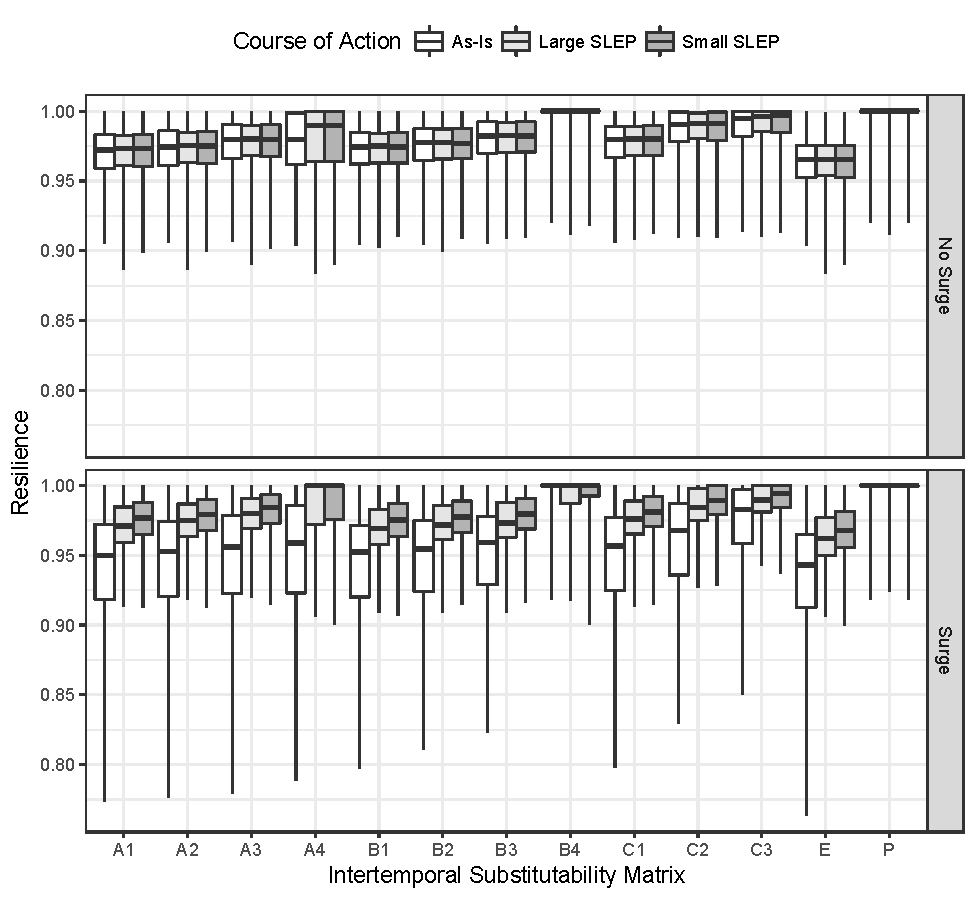
\includegraphics{CDR_Delta_GradRes}
  \caption{Commander Delta Graduate per Quarter Resilience Results for
  Each Intertemporal Substitutability Profile}
  \label{f:CO_D_Grad}
\end{figure}

\begin{figure}[h]
  \centering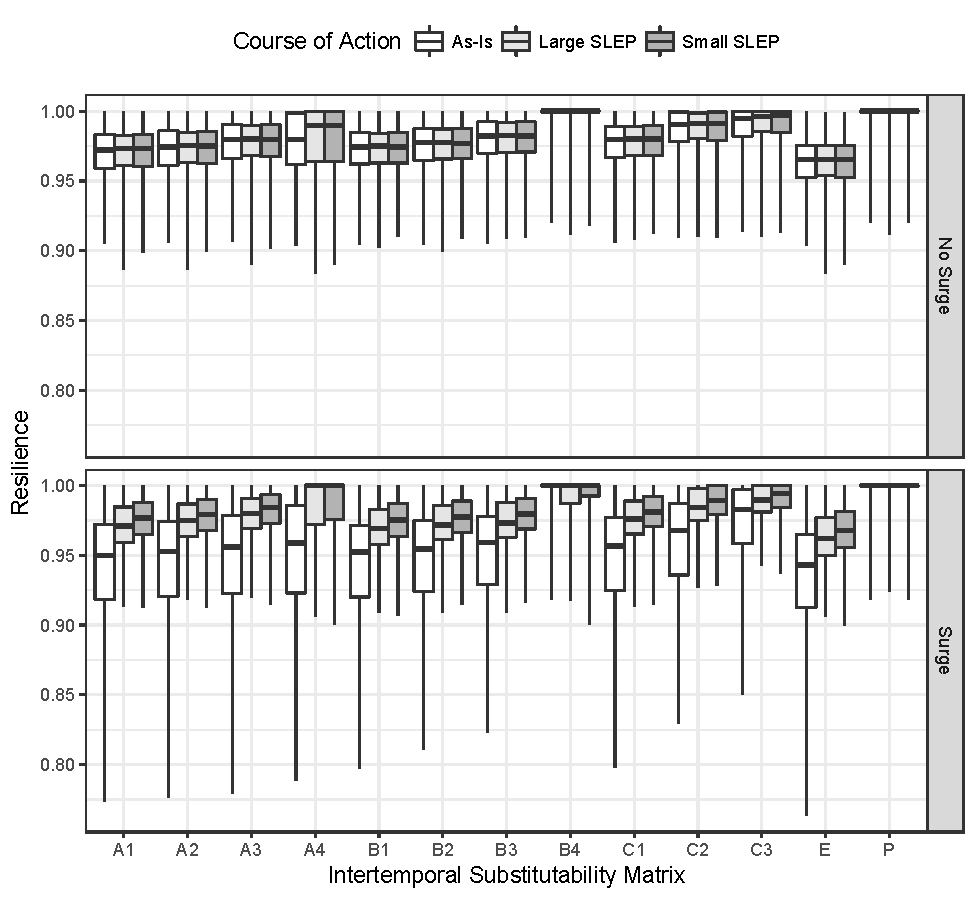
\includegraphics{CDR_Echo_GradRes}
  \caption{Commander Echo Resilience Results for
  Each Intertemporal Substitutability Profile}
  \label{f:CO_E_Grad}
\end{figure}

\section{Discussion}
\label{s:Disc}

\subsection{Hybrid Resilience Framework Demonstration}
The study applied a hybrid resilience framework to a flight training
squadron. The framework produced nuanced results to inf. The 
preferred most-resilient solution varied from stakeholder to
stakeholder and within stakeholders from output to output.

The results show resilience to be dependent upon time horizon for the
program manager. With no delay in fielding a replacement system, the
``As-Is'' course of action has the highest resilience in ready
aircraft and student satisfaction. From 20-30 years, ``As-Is'' becomes
untenable, and the ``Small SLEP'' course of action has a slight
advantage over the ``Large SLEP'' course of action. The
``Large SLEP'' is the only tenable course of action at 35 years. The
program manager would also look at resilience from the Commanding
Officers' perspective. The program manager should avoid courses of action that makes it impossible for
a Commanding Officer to meet their quotas. Figure~\ref{f:CO_Sat} shows
the sacrifice the Commanding Officers would make. The ``As-Is'' course
of action almost guarantees meeting the student satisfaction goals
with ``Small SLEP'' and ``Large SLEP'' becoming worse.

\subsection{Intertemporal Substitutability Algorithm Demonstration}

The study demonstrated a novel intertemporal substitutability
algorithm. The algorithm enables time and event dependent
surplus substitutability. The algorithm prepped the graduates per
quarter time-series data for the resilience analytical model. Figures
~\ref{f:PMGradTimeHorizon15}-~\ref{f:PMGradTimeHorizon35},
~\ref{f:PMGradAllChiPlotTimeHorizon15}-~\ref{f:PMGradAllChiPlotTimeHorizon35},
and ~\ref{f:CDR_Delta_GradRes}-~\ref{f:CDR_Echo_GradRes} show these 
results. The algorithm differentiates between surplus before and after
a shortfall. The \emph{permanent} case showed little decision support
when a course of action was viable
(Figures~\ref{PMGradAllChiPlotTimeHorizon15},
~\ref{PMGradAllChiPlotTimeHorizon20},
~\ref{PMGradAllChiPlotTimeHorizon30},
~\ref{PMGradAllChiPlotTimeHorizon30}) as the bulk of the resilience
values went to one.  The intertemporal substitutability case-to-case
change in resilience is evident from the figures. The trend fits with
intuition with an increasing trend when more time steps 
surplus percentage are available to transfer.

\subsection{Future Work}

The focus of this study was resilience. The hybrid resilience
framework provides many aides to a decision-maker considering multiple
stakeholders and outputs of interest.
One key push for future work would be to explore the parameters that
were held constant in this study for the purpose of demonstrating the
framework. Future work would look at varying more of the model parameters,
introducing variable and multiple student surge production, and
statistics for loss of aircraft. 

\subsubsection{Resilience Analysis}
This study and earlier works have developed the concept of
intertemporal substitutability. 

Randomizing the size, length, and number of student surge periods. 


%% \section{}
%% \label{}

%% References
%%
%% Following citation commands can be used in the body text:
%% Usage of \cite is as follows:
%%   \cite{key}          ==>>  [#]
%%   \cite[chap. 2]{key} ==>>  [#, chap. 2]
%%   \citet{key}         ==>>  Author [#]

%% References with bibTeX database:
\clearpage
\bibliographystyle{model1-num-names}
\bibliography{Mendeley}

%% Authors are advised to submit their bibtex database files. They are
%% requested to list a bibtex style file in the manuscript if they do
%% not want to use model1-num-names.bst.

%% References without bibTeX database:

% \begin{thebibliography}{00}

%% \bibitem must have the following form:
%%   \bibitem{key}...
%%

% \bibitem{}

% \end{thebibliography}

\end{document}

%%
%% End of file `elsarticle-template-1-num.tex'.
